\documentclass[a4paper,11pt,fleqn,dvipsnames,oneside,openright]{memoir} 	%
% Openright aabner kapitler paa hoejresider (openany begge)
%\newcommand*{\docroot}{.}%Sætter relativ rod af dokumentet
% ¤¤ Oversaettelse og tegnsaetning ¤¤ %
\usepackage[utf8]{inputenc}					% Input-indkodning af tegnsaet (UTF8)
\usepackage[danish]{babel}					% Dokumentets sprog
\usepackage[T1]{fontenc}					% Output-indkodning af tegnsaet (T1)
\usepackage{ragged2e,anyfontsize}			% Justering af elementer
%\usepackage{fixltx2e}						% Retter forskellige fejl i LaTeX-kernen

\usepackage{lmodern}

\usepackage{datetime} % Nuværende tidspunkt

% ¤¤ Figurer og tabeller (floats) ¤¤ %
\usepackage{graphicx} 						% Haandtering af eksterne billeder (JPG, PNG, EPS, PDF)s
%\usepackage{eso-pic}						% Tilfoej billedekommandoer paa hver side
\usepackage{wrapfig}						% Indsaettelse af figurer omsvoebt af tekst. \begin{wrapfigure}{Placering}{Stoerrelse}
%\usepackage{subcaption}					% Included i memoir class

\usepackage{multirow}                		% Fletning af raekker og kolonner (\multicolumn og \multirow)
\usepackage{multicol}         	        	% Muliggoer output i spalter
\usepackage{rotating}						% Rotation af tekst med \begin{sideways}...\end{sideways}
\usepackage{colortbl} 						% Farver i tabeller (fx \columncolor og \rowcolor)
\usepackage{xcolor}							% Definer farver med \definecolor. Se mere: http://en.wikibooks.org/wiki/LaTeX/Colors
\usepackage{flafter}						% Soerger for at floats ikke optraeder i teksten foer deres reference
\let\newfloat\relax 						% Justering mellem float-pakken og memoir
\usepackage{float}							% Muliggoer eksakt placering af floats, f.eks. \begin{figure}[H]
\usepackage{longtable} %Long tables

\usepackage{afterpage} %Bruges til at få billeder og figurer til at være samen med kapitlet de hører til
\usepackage{placeins}

% ¤¤ Matematik mm. ¤¤
\usepackage{amsmath,amssymb,stmaryrd} 		% Avancerede matematik-udvidelser
\usepackage{mathtools}						% Andre matematik- og tegnudvidelser
\usepackage{textcomp}                 		% Symbol-udvidelser (f.eks. promille-tegn med \textperthousand )
\usepackage{rsphrase}						% Kemi-pakke til RS-saetninger, f.eks. \rsphrase{R1}
\usepackage[version=3]{mhchem} 				% Kemi-pakke til flot og let notation af formler, f.eks. \ce{Fe2O3}
\usepackage{siunitx}						% Flot og konsistent praesentation af tal og enheder med \si{enhed} og \SI{tal}{enhed}
\sisetup{locale=DE}							% Opsaetning af \SI (DE for komma som decimalseparator) 

% ¤¤ Referencer og kilder ¤¤ %
\usepackage[danish]{varioref}				% Muliggoer bl.a. krydshenvisninger med sidetal (\vref)
%\usepackage{natbib}							% Udvidelse med naturvidenskabelige citationsmodeller
%\usepackage{xr}							% Referencer til eksternt dokument med \externaldocument{<NAVN>}
%\usepackage{glossaries}					% Terminologi- eller symbolliste (se mere i Daleifs Latex-bog)

% ¤¤ Misc. ¤¤ %
\usepackage{lipsum}							% Dummy text \lipsum[..]
\usepackage[shortlabels]{enumitem}			% Muliggoer enkelt konfiguration af lister
\usepackage{pdfpages}						% Goer det muligt at inkludere pdf-dokumenter med kommandoen \includepdf[pages={x-y}]{fil.pdf}

%EMF to PDF conversion
\usepackage{epstopdf}

% Kommentarer og rettelser med \fxnote. Med 'final' i stedet for 'draft' udloeser hver note en error i den faerdige rapport.
\usepackage[footnote,danish,final,nomargin]{fixme}

% Microtype gør at teksten ser pænere ud.
\usepackage{microtype}

\usepackage{listings}
\usepackage{titlesec}
%Usecase and accepttest numbering
%% Se http://en.wikibooks.org/wiki/LaTeX/Counters http://en.wikibooks.org/wiki/LaTeX/Labels_and_Cross-referencing og http://en.wikibooks.org/wiki/LaTeX/Macros for info på hvordan nedenståen er opstået

\newcounter{usecases} %counter
\newcommand{\usecaseset}[1]{\#\refstepcounter{usecases}\arabic{usecases}\label{usecase:#1}} %Tacking an usecase
\newcommand{\usecaseref}[1]{\ref{usecase:#1}} %referencing a usecase

\newcounter{accepttests} %counter
\newcommand{\accepttestset}[1]{\#\refstepcounter{accepttests}\arabic{accepttests}\label{accepttest:#1}}
\newcommand{\accepttestref}[1]{\ref{accepttest:#1}}

%Inkludering af class diagram
\newcommand{\includeclassdiagram}[2]{\includegraphics[width=#1,clip=true,trim=39
40 39 40]{#2}}

%Ens navne på x10 enheder
\newcommand{\xti}{X10}
\newcommand{\xtic}{X10-controller}
\newcommand{\xtie}{X10-enhed}
\newcommand{\xtis}{X10-slave}

\newsubfloat{figure}

%%%% CUSTOM SETTINGS %%%%

\pdfoptionpdfminorversion=6					% Muliggoer inkludering af pdf dokumenter, af version 1.6 og hoejere
\pretolerance=2500 							% Justering af afstand mellem ord (hoejt tal, mindre orddeling og mere luft mellem ord)

% ¤¤ Marginer ¤¤ %
\setlrmarginsandblock{3.5cm}{2.5cm}{*}		% \setlrmarginsandblock{Indbinding}{Kant}{Ratio}
\setulmarginsandblock{2.5cm}{3.0cm}{*}		% \setulmarginsandblock{Top}{Bund}{Ratio}
\checkandfixthelayout 						% Oversaetter vaerdier til brug for andre pakker

%	¤¤ Afsnitsformatering ¤¤ %
\setlength{\parindent}{0mm}           		% Stoerrelse af indryk
\setlength{\parskip}{3mm}          			% Afstand mellem afsnit ved brug af double Enter
\linespread{1,1}							% Linie afstand

% ¤¤ Litteraturlisten ¤¤ %
%\bibpunct[,]{[}{]}{;}{a}{,}{,} 				% Definerer de 6 parametre ved Harvard
% henvisning (bl.a. parantestype og seperatortegn) \bibliographystyle{bibtex/harvard}			% Udseende af litteraturlisten.
\bibliographystyle{plain}			% Udseende af litteraturlisten.

% ¤¤ Indholdsfortegnelse ¤¤ %
\setsecnumdepth{subsection}		 			% Dybden af nummerede overkrifter (part/chapter/section/subsection)
\maxsecnumdepth{subsection}					% Dokumentklassens graense for nummereringsdybde
\settocdepth{subsection} 					% Dybden af indholdsfortegnelsen

% ¤¤ Lister ¤¤ %
\setlist{
  topsep=0pt,								% Vertikal afstand mellem tekst og listen
  itemsep=-1ex,								% Vertikal afstand mellem items
} 

% ¤¤ Visuelle referencer ¤¤ %
\usepackage[colorlinks]{hyperref}			% Danner klikbare referencer (hyperlinks) i dokumentet.
\hypersetup{colorlinks = true,				% Opsaetning af farvede hyperlinks (interne links, citeringer og URL)
    linkcolor = black,
    citecolor = black,
    urlcolor = black
}

% % Sprog opsætning for referencer
\def\figureautorefname{Figur}
\def\tableautorefname{Tabel}

% ¤¤ Opsaetning af figur- og tabeltekst ¤¤ %
\captionnamefont{\small\bfseries\itshape}	% Opsaetning af tekstdelen ('Figur' eller 'Tabel')
\captiontitlefont{\small}					% Opsaetning af nummerering
\captiondelim{. }							% Seperator mellem nummerering og figurtekst
\hangcaption								% Venstrejusterer flere-liniers figurtekst under hinanden
\captionwidth{\linewidth}					% Bredden af figurteksten
\setlength{\belowcaptionskip}{10pt}			% Afstand under figurteksten
		
% ¤¤ Navngivning ¤¤ %
\addto\captionsdanish{
	\renewcommand\appendixname{Appendiks}
	\renewcommand\contentsname{Indholdsfortegnelse}	
	\renewcommand\appendixpagename{Appendiks}
	\renewcommand\appendixtocname{Appendiks}
	\renewcommand\cftchaptername{\chaptername~}				% Skriver "Kapitel" foran kapitlerne i indholdsfortegnelsen
	\renewcommand\cftappendixname{\appendixname~}			% Skriver "Appendiks" foran appendiks i indholdsfortegnelsen
}

% ¤¤ Kapiteludssende ¤¤ %
\definecolor{numbercolor}{gray}{0.7}		% Definerer en farve til brug til kapiteludseende
\newif\ifchapternonum

\makechapterstyle{jenor}{					% Definerer kapiteludseende frem til ...
  \renewcommand\beforechapskip{0pt}
  \renewcommand\printchaptername{}
  \renewcommand\printchapternum{}
  \renewcommand\printchapternonum{\chapternonumtrue}
  \renewcommand\chaptitlefont{\fontfamily{pbk}\fontseries{db}\fontshape{n}\fontsize{25}{35}\selectfont\raggedleft}
  \renewcommand\chapnumfont{\fontfamily{pbk}\fontseries{m}\fontshape{n}\fontsize{1in}{0in}\selectfont\color{numbercolor}}
  \renewcommand\printchaptertitle[1]{%
    \noindent
    \ifchapternonum
    \begin{tabularx}{\textwidth}{X}
    {\let\\\newline\chaptitlefont ##1\par} 
    \end{tabularx}
    \par\vskip-2.5mm\hrule
    \else
    \begin{tabularx}{\textwidth}{Xl}
    {\parbox[b]{\linewidth}{\chaptitlefont ##1}} & \raisebox{-15pt}{\chapnumfont \thechapter}
    \end{tabularx}
    \par\vskip2mm\hrule
    \fi
  }
}											% ... her

\chapterstyle{jenor}						% Valg af kapiteludseende - Google 'memoir chapter styles' for alternativer

% ¤¤ Sidehoved ¤¤ %

\makepagestyle{AAU}							% Definerer sidehoved og sidefod udseende frem til ...
\makepsmarks{AAU}{%
	\createmark{chapter}{left}{shownumber}{}{. \ }
	\createmark{section}{right}{shownumber}{}{. \ }
	\createplainmark{toc}{both}{\contentsname}
	\createplainmark{lof}{both}{\listfigurename}
	\createplainmark{lot}{both}{\listtablename}
	\createplainmark{bib}{both}{\bibname}
	\createplainmark{index}{both}{\indexname}
	\createplainmark{glossary}{both}{\glossaryname}
}
\nouppercaseheads											% Ingen Caps oenskes

\makeevenhead{AAU}{Aarhus Universitet - Gruppe 08}{}{\leftmark}				% Definerer lige siders sidehoved (\makeevenhead{Navn}{Venstre}{Center}{Hoejre})
\makeoddhead{AAU}{\rightmark}{}{Gruppe 08 - Aarhus Universitet}		% Definerer ulige siders sidehoved (\makeoddhead{Navn}{Venstre}{Center}{Hoejre})
\makeevenfoot{AAU}{\thepage}{}{}							% Definerer lige siders sidefod (\makeevenfoot{Navn}{Venstre}{Center}{Hoejre})
\makeoddfoot{AAU}{}{}{\thepage}								% Definerer ulige siders sidefod (\makeoddfoot{Navn}{Venstre}{Center}{Hoejre})
\makeheadrule{AAU}{\textwidth}{0.5pt}						% Tilfoejer en streg under sidehovedets indhold
\makefootrule{AAU}{\textwidth}{0.5pt}{1mm}					% Tilfoejer en streg under sidefodens indhold

\copypagestyle{AAUchap}{AAU}								% Sidehoved for kapitelsider defineres som standardsider, men med blank sidehoved
\makeoddhead{AAUchap}{}{}{}
\makeevenhead{AAUchap}{}{}{}
\makeheadrule{AAUchap}{\textwidth}{0pt}
\aliaspagestyle{chapter}{AAUchap}							% Den ny style vaelges til at gaelde for chapters
															% ... her
															
\pagestyle{AAU}												% Valg af sidehoved og sidefod


%%%% CUSTOM COMMANDS %%%%

% ¤¤ Billede hack ¤¤ %
\newcommand{\figur}[4]{
		\begin{figure}[H] \centering
			\includegraphics[width=#1\textwidth]{billeder/#2}
			\caption{#3}\label{#4}
		\end{figure} 
}

% ¤¤ Specielle tegn ¤¤ %
\newcommand{\grader}{^{\circ}\text{C}}
\newcommand{\gr}{^{\circ}}
\newcommand{\g}{\cdot}


%%%% ORDDELING %%%%

\hyphenation{}

% % listings setup
\lstset{
tabsize=4,
frame=single,
columns=fullflexible,
linewidth=\textwidth
}

% % % sørg for at floats er på siden inden en ny section starter
%\newcommand{\sectionbreak}{\clearpage}
%\newcommand{\subsectionbreak}{\FloatBarrier}

%Code handling - Colors lstlisting

\lstset{language=C++,
                basicstyle=\ttfamily,
                keywordstyle=\color{blue}\ttfamily,
                stringstyle=\color{red}\ttfamily,
                commentstyle=\color{green}\ttfamily,
                morecomment=[l][\color{magenta}]{\#}
}


\title{Projektrapport}
\author{E3PRJ3 Gruppe 08}
\date{\today{} \currenttime{}}

\begin{document}
% % % Indexes % % %
%\maketitle

\frontmatter
\thispagestyle{empty}
\begin{flushright}
\vspace{2cm}


\textit{\textbf{\textsc{\HUGE Projektdokumentation 3. semester}} \\ \vspace{1cm}}

\rule{13cm}{3mm} \\ \vspace{1cm}

%\includegraphics[width=0.9\textwidth]{billeder/forside.jpg}
\vspace{1cm} 
\textsc{\Large E3PRJ3 \\
Gruppe 8 \\
IKT, Elektro \& Stærkstrøm\\
Aarhus School of Engineering\\
\vspace{0.2cm}
\date{\today{} \currenttime{}}
}
\end{flushright}


\vspace{6.5cm}


\textsc{\Large
\begin{tabular}[\widthof{Studienummer - NavnMMMMM}]{rcl}
\textbf{Studienummer} & \textbf{-} & \textbf{Navn} \\ 
20104209 & - & Andreas Laursen \\
201270024 & - & Dannie Lehmann \\
10253 & - & Jens Rix Jørgensen \\
201270725 & - & Mathias Jessen \\
20062548 & - & Morten Møller Christensen \\
201303580 & - & Simon Mouridsen \\
201270943 & - & Stine Skaarup Høgsberg \\
\\
Vejleder & - & Lars G. Johansen
\end{tabular}
}
%\clearpage
%\chapter*{Deltageres underskrift}

\phantom{Luft}

\phantom{Luft}

\begin{table}[H]
	\centering
		\begin{tabular}{c c c}
		&&\\
		&&\\
		&&\\
		&&\\
			\underline{\phantom{mmmmmmmmmmmmmm}} && \underline{\phantom{mmmmmmmmmmmmmm}} \\
			Andreas Laursen && Dannie Lehmann\\
			20104209 && 201270024\\
			&&\\
			&&\\
			&&\\
			&&\\
			&&\\
			\underline{\phantom{mmmmmmmmmmmmmm}} && \underline{\phantom{mmmmmmmmmmmmmm}} \\
			Jens Rix Jørgensen && Mathias Jessen\\
			10253 && 201270725\\
			&&\\
			&&\\
			&&\\
			&&\\
			&&\\
			\underline{\phantom{mmmmmmmmmmmmmm}} && \underline{\phantom{mmmmmmmmmmmmmm}} \\
			Morten Møller Christensen && Simon Mouridsen\\
			20062548 && 201303580\\
			&&\\
			&&\\
			&&\\
			&&\\
			&&\\
		 							& \underline{\phantom{mmmmmmmmmmmmmm}} 	&			\\														
									& Stine Skaarup Høgsberg\\
									& 201270943								
		\end{tabular}
\end{table}

\clearpage
\chapter*{Deltageres underskrift}

\phantom{Luft}

\phantom{Luft}

\begin{table}[H]
	\centering
		\begin{tabular}{c c c}
		&&\\
		&&\\
		&&\\
		&&\\
			\underline{\phantom{mmmmmmmmmmmmmm}} && \underline{\phantom{mmmmmmmmmmmmmm}} \\
			Andreas Laursen && Dannie Lehmann\\
			20104209 && 201270024\\
			&&\\
			&&\\
			&&\\
			&&\\
			&&\\
			\underline{\phantom{mmmmmmmmmmmmmm}} && \underline{\phantom{mmmmmmmmmmmmmm}} \\
			Jens Rix Jørgensen && Mathias Jessen\\
			10253 && 201270725\\
			&&\\
			&&\\
			&&\\
			&&\\
			&&\\
			\underline{\phantom{mmmmmmmmmmmmmm}} && \underline{\phantom{mmmmmmmmmmmmmm}} \\
			Morten Møller Christensen && Simon Mouridsen\\
			20062548 && 201303580\\
			&&\\
			&&\\
			&&\\
			&&\\
			&&\\
		 							& \underline{\phantom{mmmmmmmmmmmmmm}} 	&			\\														
									& Stine Skaarup Høgsberg\\
									& 201270943								
		\end{tabular}
\end{table}

\chapter{Resumé}
Der er i forbindelse med semester projektet forsøgt at realisere en rugemaskine, i første omgang med udrugning af hønseæg i fokus. 

I projektets startforløb, er der anvendt forskellige UML og SysML værktøjer til at give overblik over projektet, og der er i denne periode anvendt en form for V-model som arbejdsmetode. I projektes design og implementerings fase er der forsøgt at anvende arbejdsmetoden Scrum.

Der er i projektet blevet anvendt to systemer, den ene, en microcontroller af typen PSoC3, og den anden, et embedded system, DevKit8000. De to systemer har i projektet skulle kommunikere med hinanden via SPI.

Til PSoC3 er der primært fokuseret på at anvende forskellige I2C sensorer, reguleringssløjfer samt kontrollere DC- og step-motorer. Disse forskellige komponenter er der blevet arbejdet med, både hardware of software mæssigt. Softwaren der er skrevet til PSoC3, er skevet i programmerings sproget C, og der er anvendt programmet PSoC Creator.

Det embeddede system, DevKit8000 et sat op med et Linux baseret operativ system. Til DevKit8000 er der udarbejdet en driver, i form af et Linux kerne modul, til at håndtere SPI kommunikationen til PSoC3, samt en interruptlinie. Derudover er der blevet lavet en GUI applikation, som har skulle benytte den førnævnte driver til at vise/sende data fra/til PSoC3. Applikationen er skrevet i C++ og anvender Qt frameworket.

Projektet involverede regulering af temperatur og luftfugtighed. Til regulering af temperatur er anvendt et PWM styret varmelegeme, og til luftfugtighedsregulering anvendes en forstøver styret af en magnetventil. 





\chapter{Abstract}
In the semester project we sought to develop a hatching machine, initially with the hatching of chicken eggs in focus.

During the start of the project, there were used various UML and SysML tools to provide an overview of the project. During this period the develop metode, V - model  was used. In the project's design and implementation phase it was attempted to apply the working method Scrum.

The project involves two systems, one of them, a microcontroller of the type PSoC3, the other an embedded system, DevKit8000. Part of the project, was to make the two systems communicate via SPI.

For PSoC3 the primary focus was on applying different types of I2C sensors, control loops as well as controlling DC- and stepper motors. These components have been worked with both hardware of software wise. The software written to PSoC3, was written in the programming language C, and the program PSoC Creator was used.

The embedded system, DevKit8000, was set up with a Linux based operating system. For the DevKit8000 a driver was made, in the form of a Linux kernel module, which had to deal with the SPI communication to PSoC3 and an interrupt line. In addition, a GUI application was developed, which used the aforementioned driver to show/send data from/to the PSoC3. The application is written in C++, using the Qt framework.

The project involved regulation of temperature and humidity. For regulation of the temperature, a PWM controlled heater was used, and for regulation of the humidity, an atmomizer controlled by a solenoid valve was used.



%indholdsfortegnelse
\clearpage
\tableofcontents*

\mainmatter
\chapter{Indledning}

Dette 3. semestersprojekt går ud på at udvikle en rugesmaskine.

%Rugesmaskinen skal indeholde en grafisk brugergrænseflade, hvorpå en bruger har mulighed for at betjene systemet. Til denne brugergrænseflade bruges DevKit8000.
%Samtidig skal der benyttes sensorer, som faget I3GFV har givet kendskab til.\newline
%Som bindeled imellem DevKit8000 og de enkelte dele af rugesmaskinen bruges en PSoC 3. Denne PSoC står for at styre selve udrugningssekvensen.

Projektet er underlagt nogle krav, specificeret i det udleverede projektoplæg:

\begin{itemize}
\item Systemet skal via sensorer/aktuatorer interagere med omverdenen
\item Systemet skal have brugerinteraktion
\item Systemet skal indeholde faglige elementer fra semesterets andre fag.
\item Systemet skal anvende DevKit8000 og PSoC3 teknologi.
\end{itemize}

Ydermere er der følgende fokuspunkter:
\begin{itemize}
\item Udarbejdelse af et abstract rettet mod eksterne folk om projektet.
\item Implementering og test af et udviklingsprojekt med både HW og SW, der integrerer semesterets
kurser.
\item Definition af en kravspecifikation for projektet.
\item Samarbejde i grupper med både HW og SW udviklerroller
\item Arbejdsmetode orienteret mod at udvikle nye produkter baseret på HW og SW.
\end{itemize}


%\section{Rapportopbygning}
%Rapporten er bygget op således at de første afsnit giver et overordnet indblik i projektets formål og afgrænsninger. 
%Derefter bliver der sat fokus på kravene for projektet og design overvejelserne.
%I konklusionen på rapporten vil der være en fælles konklusion på projektet. Derudover vil hvert enkelt gruppemedelem komme med hans/hendes personlige konklusion. 
%I starten af rapporten er der inkluderet en ordliste. Denne ordliste er med for at give forståelse for nogen af de begreber der bliver brugt igennem rapporten. 



% \chapter{Tidsplan}

% \begin{figure}[h]
% \centering
% 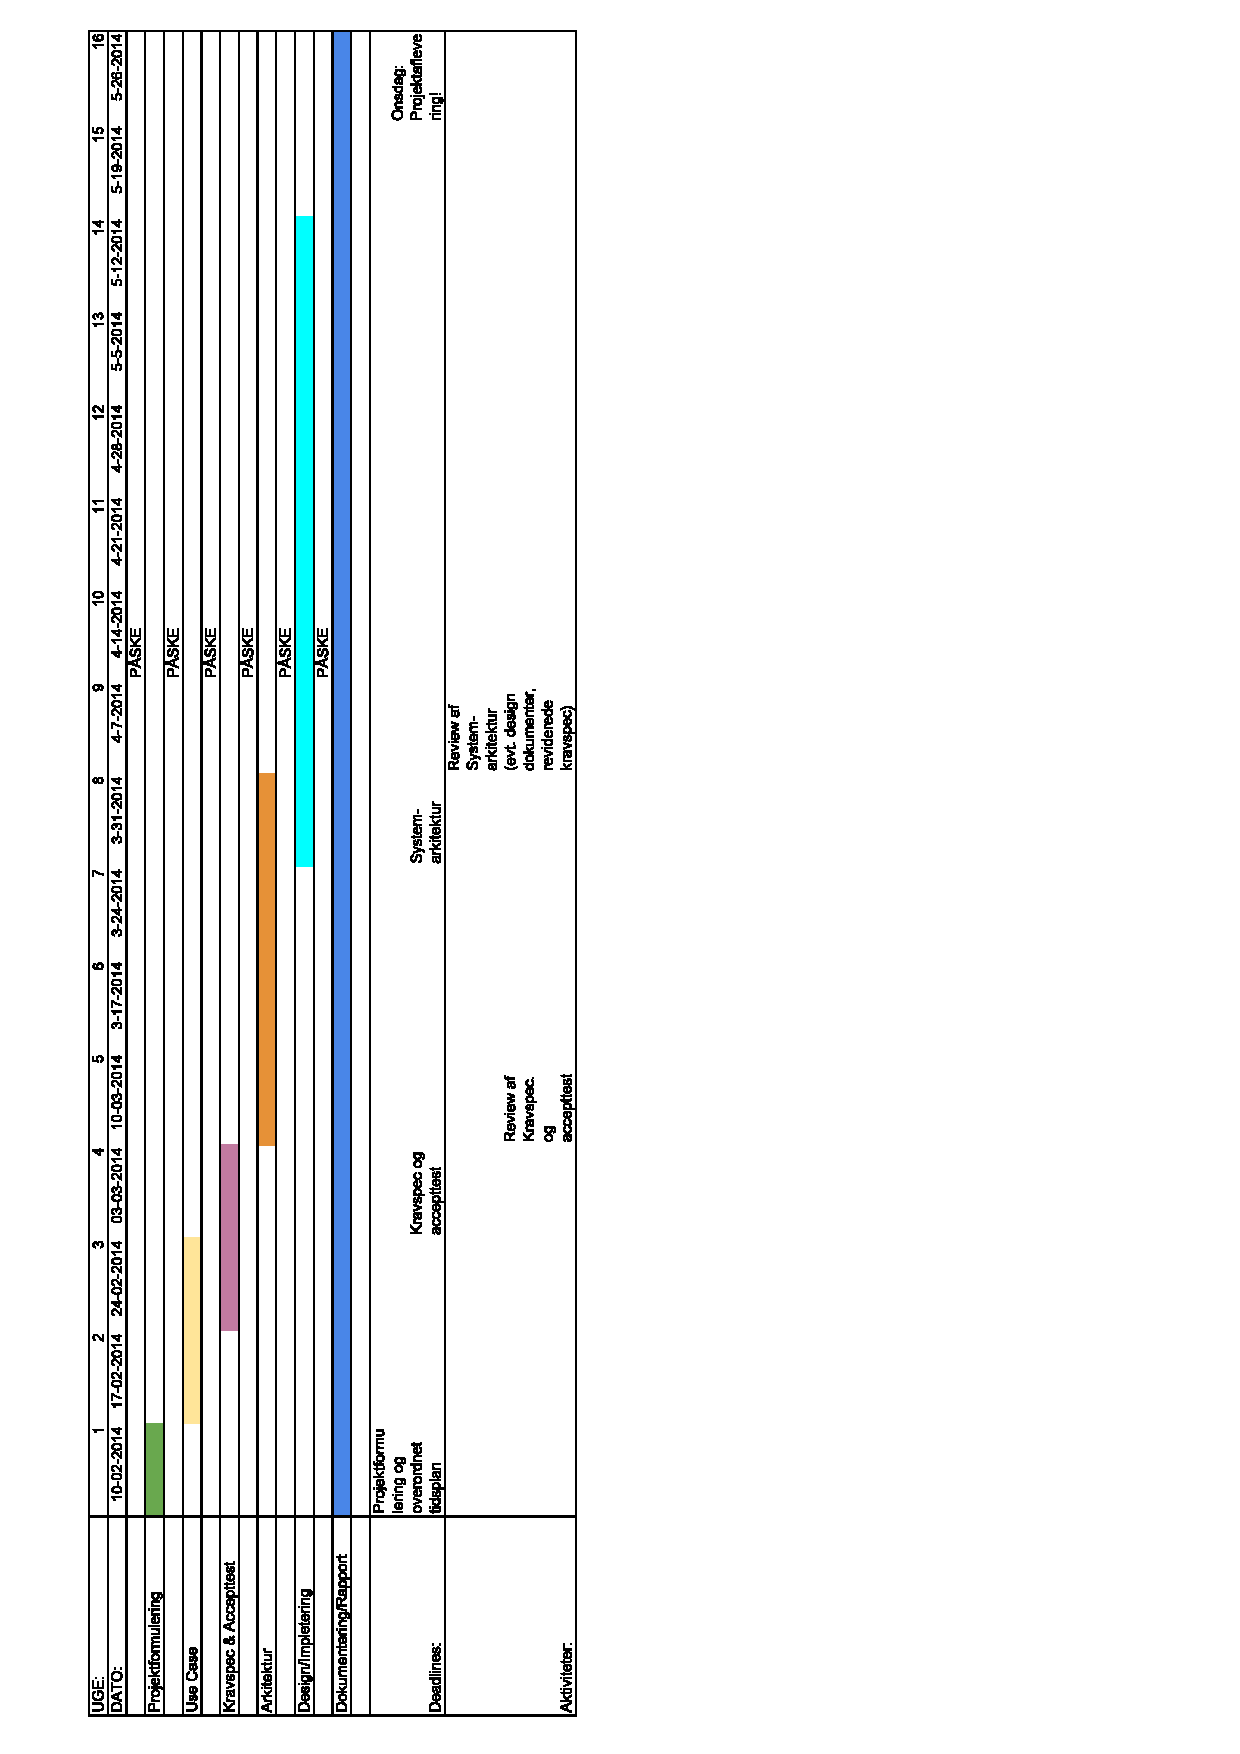
\includegraphics[scale=0.6]{2_indledning/PDFC-.pdf}
% \caption{Skitse af projekt oversigt}
% \label{fig:projektoversigt}
% \end{figure}
% \clearpage

\section{Ordliste}
%\center %affects the entire document???

Denne ordliste er med for at give forståelse for nogen af de begreber der bliver brugt igennem rapporten. 

\begin{tabular}{|l|l|}
\hline  \textbf{Ord} & \textbf{Betydning}  \\ 
\hline SysML & System Modeling Language. \\
\hline Emner & Kyllinger og æg. \\ 
\hline Maskine & Betegner de fysiske rammer. \\
\hline System & Betegner de funktionelle rammer.  \\ 
\hline Ægtype & Typen af æg, der skal udruges. \\
\hline 
\end{tabular} 

\clearpage


\chapter{Opgaveformulering}


\section{Projektformulering - Projekt rugemaskine}

Miljøstyring for en rugemaskine til udrugning af æg.

\subsection{Baggrund}

Styring af miljøet i et udrugningsmiljø er kritisk for udrugning af æg. Derfor kræver det et sensoroveråget og -styret rum, som kan justere på følgende parametre:

\begin{itemize}
\item Temperatur
\item Ventilation/udluftning
\item Fugtighed
\item Vending
\item Afkøling
\end{itemize}

Det optimale forløb for udrugningen af et hønseæg indebærer en temperatur på omkring 37 grader, at luften omkring æggene bliver udskiftet jævnligt, at fugtigheden først i forløbet er mellem 25 og 50 procent, at fugtigheden de sidste dage af udrugningen er så høj som mulig, at æggene vendes 2-3 gange dagligt, og til sidst at æggene afkøles en gang om dagen.

\subsection{Projektdefinition}
Der skal fremstilles et system til overvågning og styring af en rugekasse. Systemet skal opfylde nedenstående systemkrav:

\begin{itemize}
\item Systemet skal kontinuert overvåge og styre miljøet i rugekassen ud fra brancheanerkendte parametre, og ud fra en fastlagt procedure vende og afkøle æggene. I denne overvågning og styring skal DevKit8000 og PSoC3 indgå.
\item Brugeren skal, vha. DevKit8000, kunne interagere med systemet. 
\item Brugeren skal, vha. DevKit8000, kunne se rummets nuværende sensorstatus, herunder temperatur.
\end{itemize}
\newpage
Projektet er skitseret på figur \ref{fig:projektoversigt} 
\begin{figure}[H]
\centering
\fbox{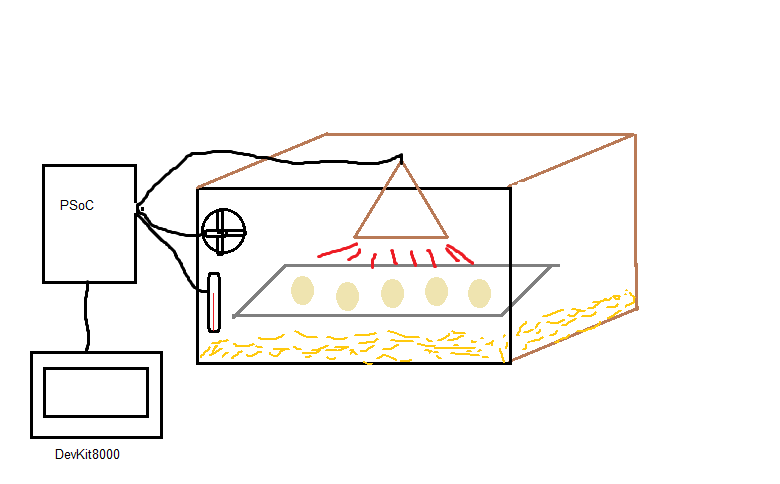
\includegraphics[scale=0.5]{3_opgaveformulering/Unavngivet.png}}
\caption{Skitse af projekt oversigt}
\label{fig:projektoversigt}
\end{figure}


\chapter{Projektafgrænsning}

%Beskrivelse af projektet set i en større kontekst og de afgrænsninger man har valgt for projektet (prototype, færdiggørelse, udformning osv. osv.). Hvis der er specificeret eller designet mere end implementeret i jeres prototype beskrives det i dette afsnit.


Der er fra projektgruppens side valgt at kører hele projektet digitalt, og derved kunne der undgås at tage stillingen til for meget støj på signalerne. 

Systemet er oprindeligt tænkt til at kunne håndtere flere forskellige typer af æg. Det er valgt at fokusere på kun een type, da dette illustrerer funktionaliteten af systemet, og udvidelse kan udføres på basis af denne prototype.

Følgende ting bliver beskrevet som del af systemet, men er ikke blevet implementeret:

- Den mekaniske del af mekanismen til vending af æg. Mekanismen blev bedømt til ikke at være nødvendig for at demonstrere funktionen til at vende æg, da dette kan illustreres ved at stepmotoren drejer rundt. Hvad angår valget af motor til vendemekanismen, er der ikke taget yderligere forudsætninger hvad ang. moment, omdrejnings hastighed osv. Dette skyldes at det var funktionen ved en stepmotor der skulle fremvises i projektet, frem for det færdige resultat.

- De overordnede, fysiske rammer for rugemaskine, selve kassen. Dette skyldes at der vendemekanismen ikke er bleven designet/bygget, det gør at der ikke kan tages stilling til den de enelige mål. Dog er der anvendt en simple kasse (prototype), således at reguleringen har været mulig og teste. 

- Der er ikke blevet lavet en selvforsynende befugter. Dette skyldes at luftfugtigheden bliver øget ved at forstøve vand ind i rugemaskinen, og skulle der laves et system der selv kan opretholde et fast tryk til forstøvelse, vil opgaven blive for omstænding. Derfor er der fundet en løsning med en trykflaske, med dertil en pumpe som øger trykke i beholderne, som gøre det muligt at forstøve vand ind i kassen.


\chapter{Systembeskrivelse}

Udrugningssystemet vil bestå af to styringsenheder: DevKit8000 der udgør brugerens interface til systemet, og en PSoC3 der styrer udrugningen.

Derudover vil systemet bestå af sensorer til måling af temperatur og luftfugtighed, aktuatorer til påvirkning af temperatur, luftfugtighed, samt til at vende æggene. Yderligere vil en kasse udgøre miljøet hvori æggene placeres. Kassen vil desuden have en sensor til registrering af åbning og lukning af lågen.

Figur \ref{fig:BDDLogisk} på side \pageref{fig:BDDLogisk} viser systemets komponenter.

%Figur \ref{fig:SystemStateDiagram} viser systemets komponenter.


%\begin{figure}[H]
%\centering
%\includegraphics[page=1,width=\linewidth,viewport=08mm 8mm 238mm 80mm]{./5_systembeskrivelse/diagrammer/SYSML_Diagrammer_v4.pdf}
%\caption[Diagram]{Logical bdd}
%\label{fig:SystemStateDiagram}
%\end{figure}
\chapter{Krav}

\section{Generelt}
Der er i dette projekt oprettet 3 typer af krav. Der er forhåndskrav bestående af krav til brugen af platformtyper samt indhold af sensorer og/eller aktuatorer. Der er Udrugningskrav som består af fundne anbefalinger til et udrugningsforløb. Det endelige valg er taget fra hjemmesiden\footnote{Hønsehuset.dk \cite{Rugetips}}. Den sidste type af krav er personlige krav til systemets funktionalitet, det er her bl.a. kravene til tests af systemet bliver beskrevet. De personlige krav er stærkt fremkomne i de udarbejdede Use Cases, samt i nogle af de ikke funktionelle krav. Der er i rapporten valgt kun at fokusere på Use Casene, og derfor kan de ikke funktionelle krav kun findes i kravspecifikationen i dokumentationsrapporten.

\section{Use Cases}
Kravene for projektet er formuleret ved brug af Use Cases.\newline De anvendte Use Cases er illustreret på figur \ref{fig:usecase_diagram}. Denne figur viser Use Case diagrammet som blev udviklet under projektforløbet.
\begin{figure}[h]
\centering
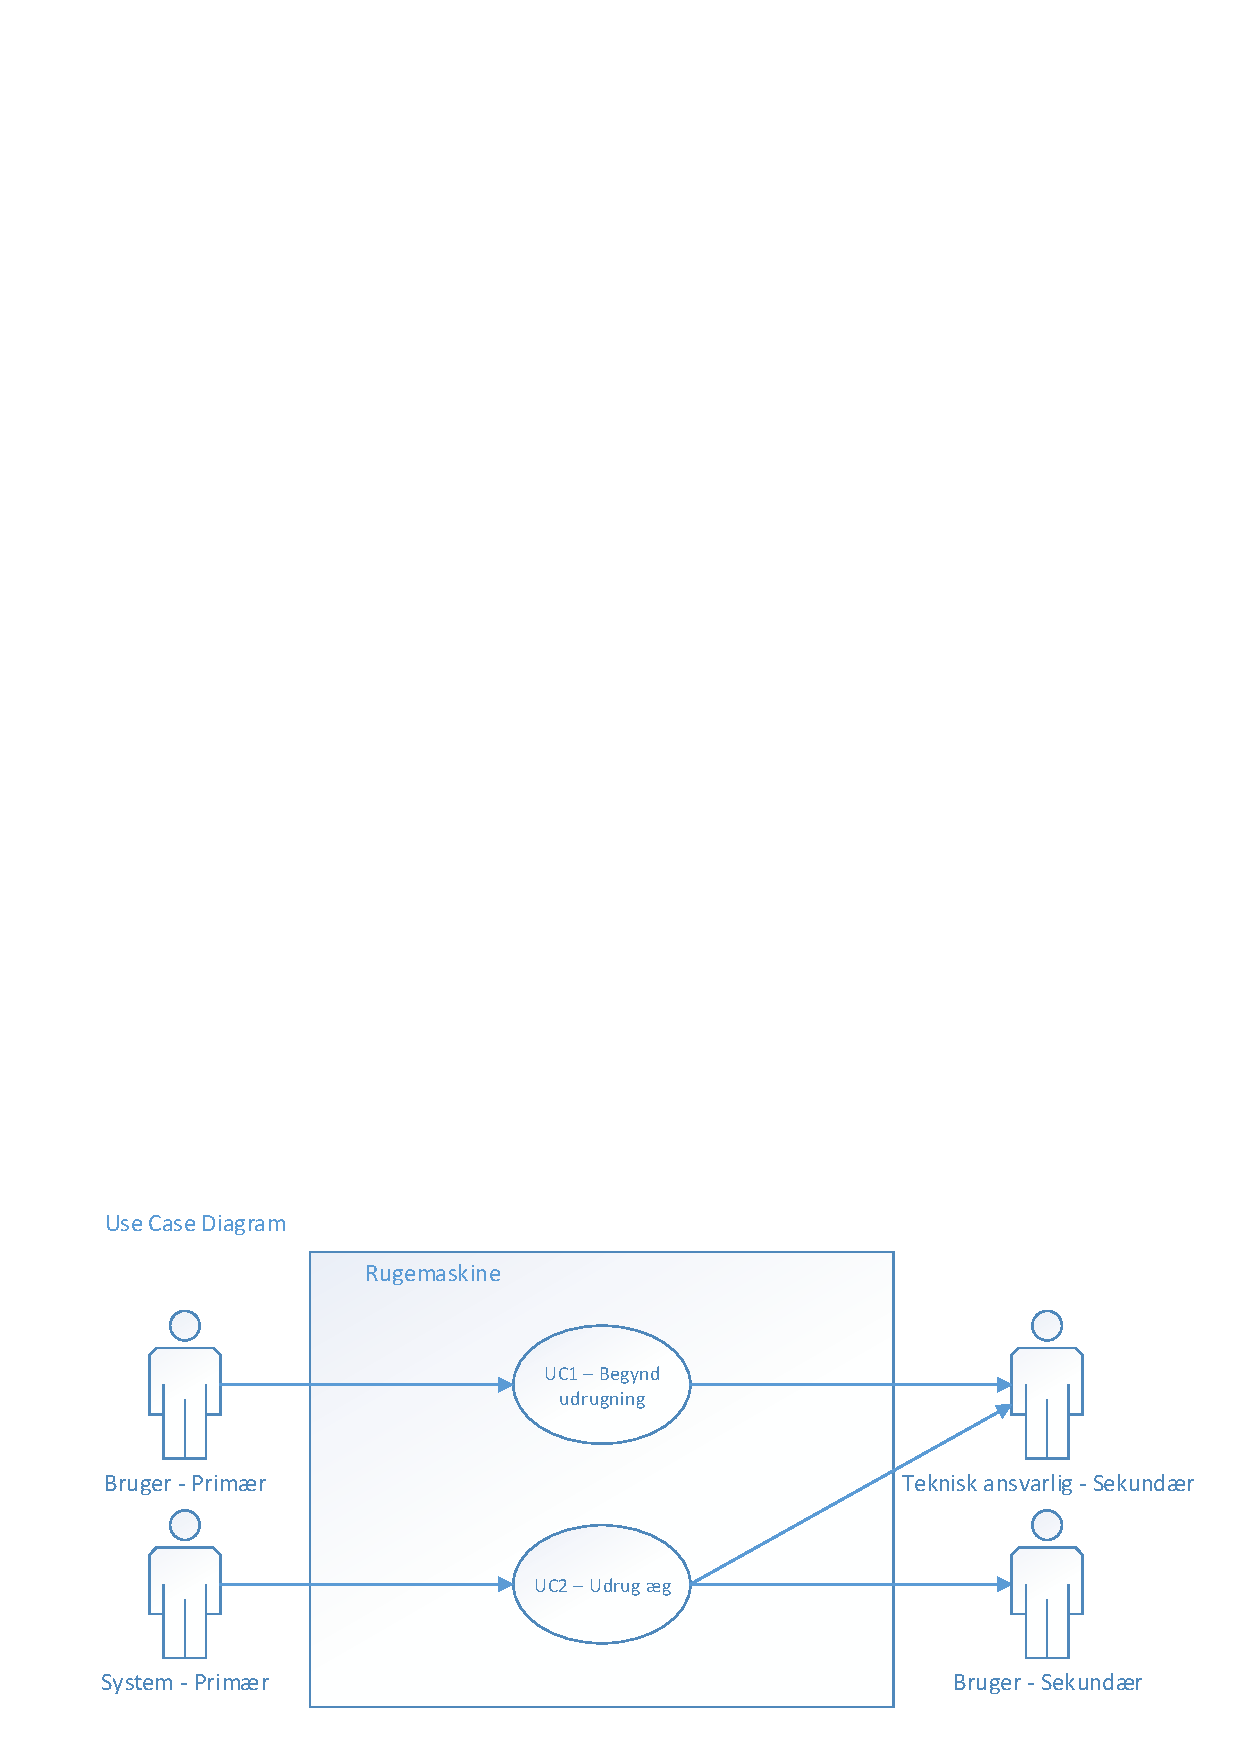
\includegraphics[width=16cm, scale=0.8, trim= 0mm 0mm 0mm 200mm, clip=true,  angle=0]{6_krav/diagrammer/UseCase_Generel_v1.pdf}
\caption{Use Case diagram}
\label{fig:usecase_diagram}
\end{figure}
\newline Det ses at de funktionelle krav er blevet opdelt i 2 Use Cases, Begynd udrugning og Udrug æg.

\textbf{Begynd udrugning:}
Denne Use Case omhandler setup processen, den er beskrevet ud fra brugerens synspunkt. Den beskriver hvorledes brugeren placerer æg i maskinen, samt den efterfølgende process hvor brugeren vælger æggetypen, og derefter starter udrugningsprocessen svarende til det trufne valg.\newline

\textbf{Udrug æg:}
Denne Use Case følger direkte efter Use Case 1, og omhandler systemets håndtering af udrugningsprocessen, samt den afsluttende fase når den ordinære process er færdiggjort. Der beskrives reguleringen af varme og fugtighed, samt hvordan der tjekkes for tidspunkter for æggevending og udluftning. I den afsluttende fase skal der stadig reguleres temperatur og luftfugtighed, men der skal ikke vendes æg.

\subsection{Aktører}
Der er til Use Casene tre vigtige aktører som interagerer med rugemaskinen:
\begin{itemize}
	\item \textbf{Bruger} \newline
	Dette er brugeren som ønsker at udruge æg. Brugeren er hovedsageligt aktiv i den indledende og afsluttende fase af udrugningen hvor der skal ilægges æg og fjernes kyllinger og/eller ikke udrugede æg.
	\item \textbf{System} \newline
	Systemet er den automatiserede styring af udrugningsprocessen. Det er systemet, der håndterer reguleringen af miljøet og styringen af aktuatorerne der er tilstede i rugemaskinen, samt grænsefladen til brugeren.
	\item \textbf{Teknisk ansvarlig} \newline
	Den tekniske ansvarlige er en person med tilstrækkelig viden om rugemaskinen til at kunne fejlfinde og reparere eventuelle fejl.
	\end{itemize}

%\chapter{Funktionelle krav}

%\section{Use Case diagram}

%\begin{figure}[h]
%\centering
%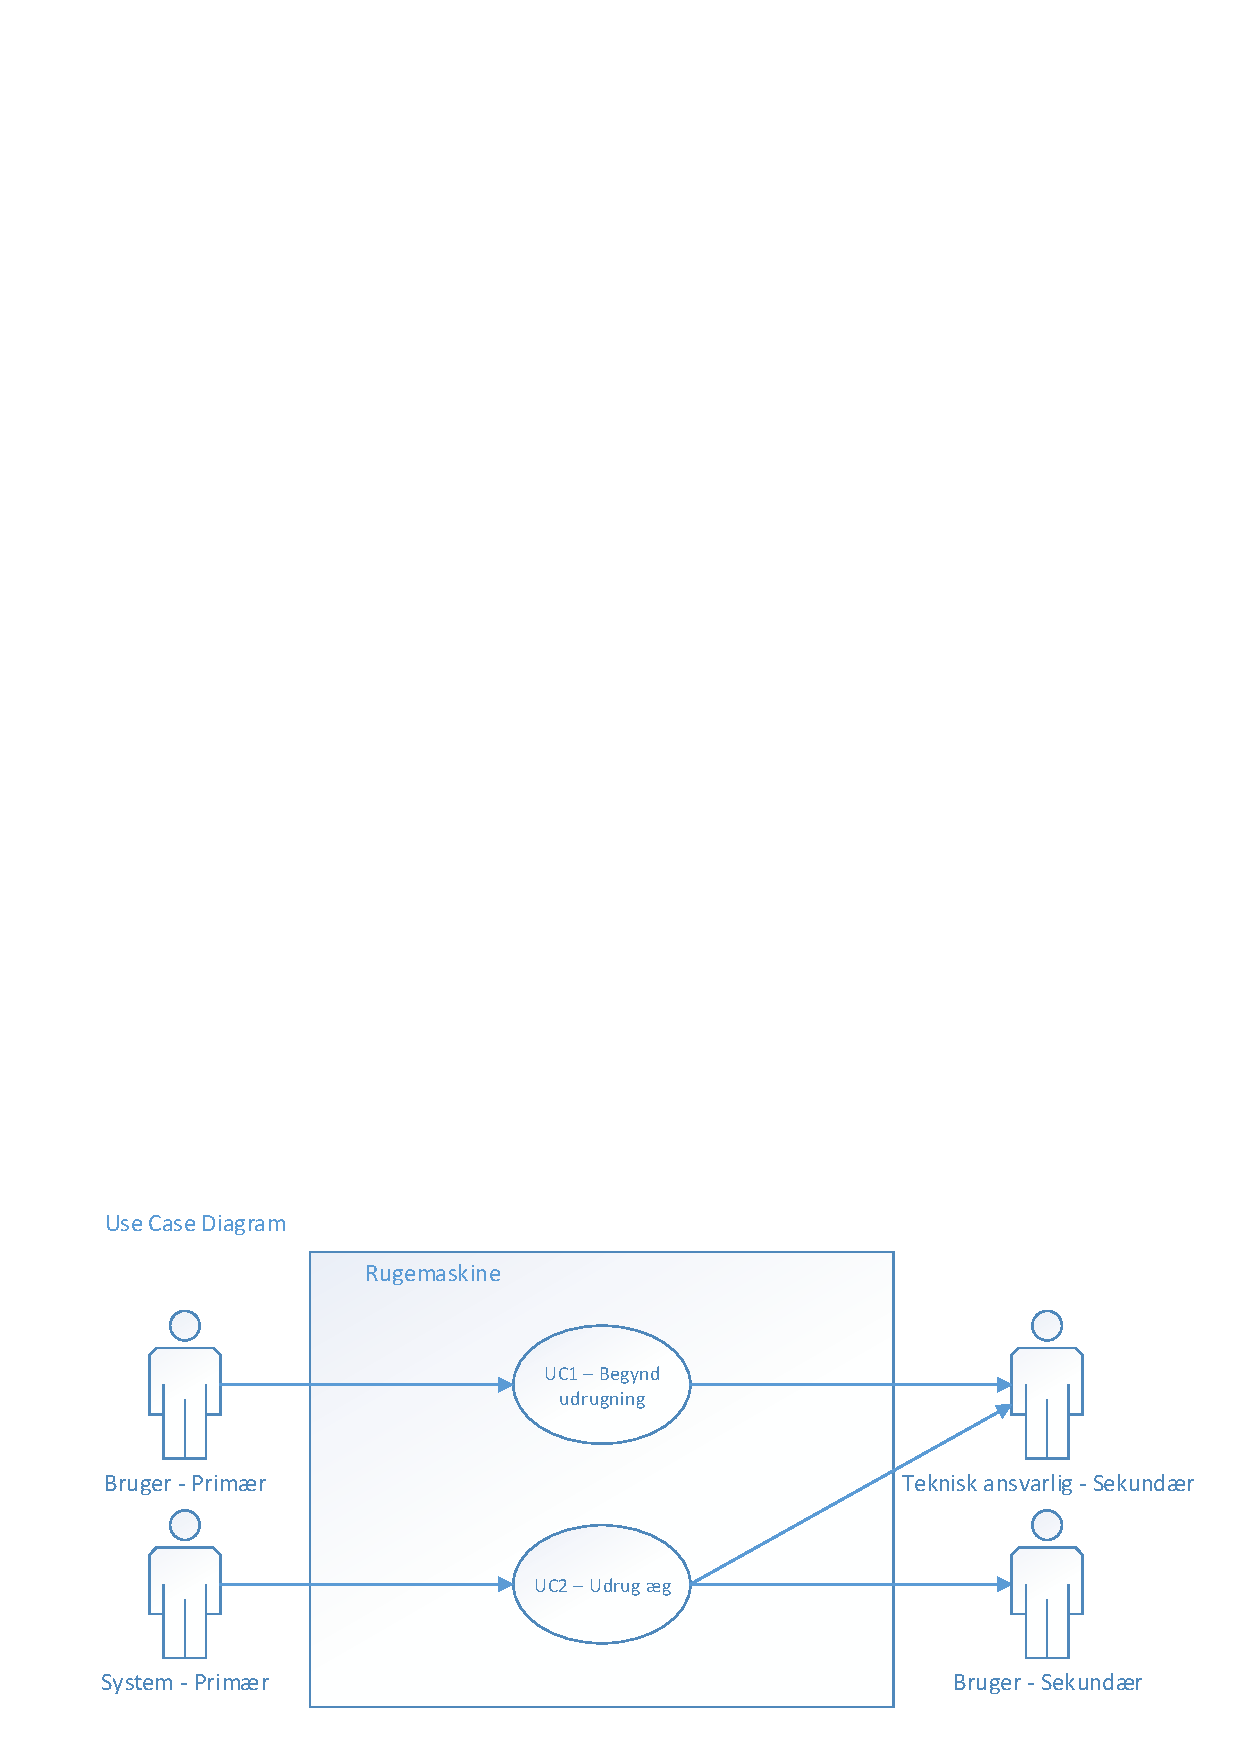
\includegraphics[width=16cm, scale=1, trim= 0mm 0mm 0mm 200mm, clip=true,  angle=0]{6_krav/diagrammer/UseCase_Generel_v1.pdf}
%\caption{Use Case diagram}
\label{fig:usecase_diagram}
%\end{figure}

%\clearpage
%\section{Aktørbeskrivelse}
%
\subsection{Bruger}

\begin{table}[H]
\centering
\begin{tabular}[\textwidth]{|p{0.20\textwidth}|p{0.80\textwidth}|}
\hline Aktørnavn: & Bruger \\ 
\hline Alternativt navn: & User \\ 
\hline Type: & Primær og sekundær\\ 
\hline Beskrivelse: & 
		\begin{enumerate}
		\item Bruger ønsker at udruge æg
		\end{enumerate} \\ 
\hline
\end{tabular}
\caption{Aktør - Bruger}
\label{tab:usecase-aktoer-bruger}
\end{table}


%
\subsection{System}

\begin{table}[H]
\centering
\begin{tabular}[\textwidth]{|p{0.20\textwidth}|p{0.80\textwidth}|}
\hline Aktørnavn: & System \\ 
\hline Alternativt navn: & Rugemaskine \\ 
\hline Type: & Primær \\ 
\hline Beskrivelse: & 
		\begin{enumerate}
		\item Systemet styrer udrugningsprocesser.
		\item Systemet har til opgave at overvåge temperatur, luftfugtighed samt tidsprogression.
		\end{enumerate} \\ 
\hline
\end{tabular}
\caption{Aktør - System}
\label{tab:usecase-aktoer-system}
\end{table}


%
\subsection{Tekniske ansvarlig}

\begin{table}[H]
\centering
\begin{tabular}[\textwidth]{|p{0.20\textwidth}|p{0.80\textwidth}|}
\hline Aktørnavn: & Tekniske ansvarlig \\ 
\hline Alternativt navn: & Servicetekniker \\ 
\hline Type: & Ekstern \\ 
\hline Beskrivelse: & 
		\begin{enumerate}
		\item Tekniske ansvarlig er en uddannet tekniker, der har en faglig forståelse for opbygning af rugemaskinen.
		\end{enumerate} \\ 
\hline
\end{tabular}
\caption{Aktør - Tekniske ansvarlig}
\label{tab:usecase-aktoer-tekniskeansvarlig}
\end{table}


%\clearpage
%\section{Use Cases}
%\subsection{Begynd udrugning}

\begin{table}[H]
\centering
\begin{tabular}[\textwidth]{|p{0.18\textwidth}|p{0.82\textwidth}|}
\hline Navn & Begynd udrugning \\ 
\hline Usecase ID & \usecaseset{Begynd udrugning} \\ 
\hline Scope &  \\
\hline Primær aktør & Bruger \\ 
\hline Interessenter & Tekniske ansvarlig. \\ 
\hline Forudsætning & Use Case \usecaseref{Udrug aeg} er ikke aktiv \\ 
\hline Resultat & Udrugning af indlagte æg er påbegyndt. \\ 
\hline Hovedforløb &
	\begin{enumerate}
	\item \label{itm:Begynd-step1} Bruger åbner låge.
	\item \label{itm:Begynd-step2} Systemet registrerer åbning af låge. 
	\item \label{itm:Begynd-step3} Systemet låser for interfacet (skriver "låge åben").
	\item \label{itm:Begynd-step4} Bruger placerer æg i maskine.
	\item \label{itm:Begynd-step5} Bruger lukker låge.
	\item \label{itm:Begynd-step6} Systemet registrerer lukning af låge.  
	\item \label{itm:Begynd-step7} Systemet låser op for interfacet (fjerner "låge åben").
	\item \label{itm:Begynd-step8} Bruger vælger type af æg til udrugning (sekvens).
	\item \label{itm:Begynd-step9} Systemet spørger bruger om bekræftelse.
	\item \label{itm:Begynd-step10} Bruger bekræfter valg (vælger "OK").
	\item \label{itm:Begynd-step11} Systemet registrerer valg.
	\item \label{itm:Begynd-step12} Systemet aktiverer sekvensen Udrug Æg (Use Case \usecaseref{Udrug aeg}).
%	\item \label{itm:Begynd-step12} 
	\end{enumerate} \\
	\hline Undtagelser &
	\begin{enumerate}
	\item[\ref{itm:Begynd-step2}a.] System registrerer ikke åbning af låge. 
	\begin{itemize}
	\item Bruger kontakter teknisk ansvarlig. 
	\end{itemize}
	\item[\ref{itm:Begynd-step6}a.] System registrerer ikke lukning af låge.  
	\begin{itemize}
	\item Bruger kontakter teknisk ansvarlig. 
	\end{itemize}
	\item[\ref{itm:Begynd-step10}a.] Bruger bekræfter ikke valg (vælger "Annullér"). 
	\begin{itemize}
	\item Step \ref{itm:Begynd-step8} gentages.
	\end{itemize}
	\end{enumerate} \\
\hline 
\end{tabular}
\caption{Use Case - Begynd udrugning}
\label{tab:usecase-Begynd-udrugning}
\end{table}
%\linespread{1.0}\subsection{Udrug {\ae}g}
\begin{table}[H]
\centering
\begin{tabular}[\textwidth]{|p{0.18\textwidth}|p{0.82\textwidth}|}
\hline Navn & Udrug æg \\ 
\hline Usecase ID & \usecaseset{Udrug aeg} \\ 
\hline Primær aktør & System \\ 
\hline Interessenter & Sekundær aktør: Bruger \\ 
\hline Forudsætning & Use Case \usecaseref{Begynd udrugning} \\ 
\hline Resultat & Æggene er udruget og fjernet fra maskinen \\ 
\hline Hovedforløb &
	\begin{enumerate}
	\item \label{itm:udrugning-step1} Systemet indlæser valgte sekvens.
	\item \label{itm:udrugning-step2} Systemet regulerer temperatur og luftfugtighed.
	\item \label{itm:udrugning-step3} Systemet kontrollerer om det er tid til æggevending.  \newline
	\textbf{hvis} (tid = æggevending): Vend æg.
	\newline
	\textbf{ellers}: Vend ikke æg.
	\newline
	Step \ref{itm:udrugning-step2}-\ref{itm:udrugning-step3} gentages indtil udrugningstiden er afsluttet.
	\item \label{itm:udrugning-step4} 	System informerer brugeren om at udrugningssekvens er færdig.
	\item \label{itm:udrugning-step5} 	Bruger åbner låge.
	\item \label{itm:udrugning-step6} 	Systemet registrerer åbning af låge.
	\item \label{itm:udrugning-step7} 	Systemet afbryder regulering af temperatur og luftfugtighed.
	\item \label{itm:udrugning-step8} 	Bruger fjerner emne(r).
	\item \label{itm:udrugning-step9} 	Bruger lukker låge.
	\item \label{itm:udrugning-step10} 	Systemet registrerer lukning af låge.
	\item \label{itm:udrugning-step11} 	Systemet genoptager regulering af temperatur og luftfugtighed.
	\newline Step \ref{itm:udrugning-step5}-\ref{itm:udrugning-step11} gentages indtil brugeren indikerer overfor systemet at alle emner er fjernet.
	\item \label{itm:udrugning-step12}		Systemet stopper med regulering af temperatur og luftfugtighed.	
	\end{enumerate} \\
\hline Undtagelser &


\begin{enumerate}
		\item[*] Bruger afbryder udrugningen.
		\begin{itemize}
			\item Systemet afbryder Use Case \usecaseref{Udrug aeg}
		\end{itemize}
	\end{enumerate}

	\begin{enumerate}
		\item[*](\ref{itm:udrugning-step2}-\ref{itm:udrugning-step3}) Bruger åbner maskinen.
		\begin{itemize}
			\item Systemet afbryder trin 2-3.
			\begin{itemize}
				\item Bruger lukker maskinen.
				\item Systemet fortsætter med trin 2-3.
			\end{itemize}
		\end{itemize}
	\end{enumerate}

	\begin{enumerate}
	\item[\ref{itm:udrugning-step2}a.] Systemet kan ikke regulere temperatur eller luftfugtighed.
	\begin{itemize}
	\item Systemet registrerer fejl.
	\item Systemet informerer bruger om fejl.
	\end{itemize}
	\end{enumerate} 
	
	
	\begin{enumerate}
	\item[\ref{itm:udrugning-step6}a.]  System registrerer ikke åbning af maskine.
	\begin{itemize}
	\item Bruger kontakter tekniske ansvarlig.
	\end{itemize}
	\end{enumerate}  
	
	\begin{enumerate}
	\item[\ref{itm:udrugning-step10}a.]  System registrerer ikke lukning af maskine.
	\begin{itemize}
	\item Bruger kontakter tekniske ansvarlig.
	\end{itemize}
	\end{enumerate} \\ \hline 
\end{tabular}
\caption{Use Case - Udrug æg}
\label{tab:usecase-Udrug-aeg}
\end{table}
%\clearpage
%\section{Funktionelle krav}
%
\begin{enumerate}
 \item Systemet skal kunne regulere temperaturen efter justering af parameter inden for 10 min. 
 \item Systemet skal kunne regulere luftfugtigheden efter justering af parameter inden for 10 min.
\end{enumerate}
\FloatBarrier

%\section{Ikke-funktionelle krav}
%
\begin{enumerate}

\item Hvis systemet ikke kan overholde de angivne grænser som er beskrevet i de funktionelle krav, skal brugeren informeres vha. alarmer.

\item DevKit8000 8000 anvendes som styrende enhed samt grafisk brugergrænseflade (GUI).

\item PSoC3 og/eller 4 anvendes som grænseflade til føler/sensorer samt aktuatorer.

\item Tilladte afvigelser:
	\begin{itemize}
	\item Temperatur: $\pm$ 1$^\circ$C.
	\item Luftfugtighed : $\pm$ 10 procentpoint.
	\end{itemize}

\item Krav til opstillingsmiljø:
	\begin{itemize}
	\item Temperatur : 15-30$^\circ$C.
	\item Luftfugtighed : <45\% procentpoint.
	\end{itemize}

\item krav til GUI:
	\begin{itemize}
	\item Der skal være mulighed for at navigere via GUI.
	\item GUI skal kunne bruges til at starte og stoppe udrugningen.
	\item Der skal altid på UI under udrugning fremgå: Temperatur, luftfugtighed, tidsprogression.
	\item GUI skal gøre bruger opmærksom på tilstandsændringer.
	\end{itemize}

\item Rugemaskinens dimensioner er: $\pm$ 2 cm
	\begin{itemize}
	\item Brede x cm
	\item Højde x cm
	\item Dybte x cm
	\end{itemize}
		
\item Udrugningsprocedurer skal følge anbefalingerne angivet på www.hønsehus.dk/opdraet/rugetips/

\item Rotation: Rotation på 180$^\circ$ $\pm$ 45$^\circ$

\end{enumerate}

%\clearpage
%\section{Accepttestspecifikation}
%Da vi ikke formåede at sammensætte og teste systemet i dets helhed, kan vi ikke godkende nedenstående accepttests. Vi har dog gennemført og godkendt flere af testene i et "subset" af systemet, som inkluderede sammensatte moduler.

\subsection{Accepttestspecfikation for Use Case \usecaseref{Begynd udrugning}} 

%************************ Use Case 1 **************************************
 
 \subsubsection{Hovedscenarie}
\begin{center}

	\begin{tabular}{| p{3cm} | p{3cm} | p{3cm} | p{3cm} |}
		\hline
		Krav & Udførelse & Forventet resultat & Resultat \\ \hline
		% % % % % % % % % % % % % % % % % % % % % % % % % % % % 
		
		\multirow{2}{3cm}{Ved lågens åbning låses UI. Det forbliver låst indtil lågen lukkes.} 
		& Maskinen står i idle tilstand og lågen åbnes
		& UI låser
		& \\ \cline{2-4}
		
		&Lågen lukkes igen
		
		&UI låser op
		& \\ \hline 
		

	\end{tabular}
\end{center}

%\subsubsection{Undtagelser}
%\begin{center} 
%	\begin{tabular}{| p{3cm} | p{3cm} | p{3cm} | p{3cm} |}
%	\end{tabular}
%\end{center}

\subsection{Accepttestspecfikation for Use Case \usecaseref{Udrug aeg}} 

%************************ Use Case 2 **************************************
 
 \subsubsection{Hovedscenarie}
\begin{center}

	\begin{longtable}{| p{3cm} | p{3cm} | p{3cm} | p{3cm} |}
		\hline
		Krav & Udførelse & Forventet resultat & Resultat \\ \hline
		% % % % % % % % % % % % % % % % % % % % % % % % % % % % 
		
		
		Systemet skal kunne regulere og holde en temperatur indenfor grænserne angivet i ikke funktionelle krav.
		&Systemet opstilles i omgivelser der ligger indenfor de påkrævede rammer. Systemet indstilles til at skulle holde 37$^\circ$C. Systemet sættes i gang og temperaturen aflæses efter 10 minutter. 
		&Maskinen kan regulere og holde temperaturen indenfor de angivne rammer. 
		& \\ \hline
		
		Systemet skal kunne regulere og holde en luftfugtighed indenfor grænserne angivet i ikke funktionelle krav.
		&Systemet opstilles i omgivelser der ligger indenfor de påkrævede rammer. Systemet indstilles til at skulle holde 70\% relativ luftfugtighed. Systemet sættes i gang og luftfugtigheden aflæses efter 10 minutter.
		&Maskinen kan regulere og holde luftfugtigheden indenfor de angivne rammer.
		& \\ \hline
		
		Maskinen kan vende æg med et bestemt interval. Æggene roteres indenfor de i ikke funktionelle krav specificerede grænser.
		&Æg-type specificeres, og systemet indstilles til at skulle vende æggene hvert 5. minut i en periode på 30 minutter. Æggenes vertikale akse markeres med en pil, der peger op. Systemet sættes i gang og kører i 30 minutter. Ved hver vending måles rotation af hvert æg, og deres rotation noteres. Efter hver rotation vendes hvert æg manuelt så orienteringsindikatoren (pilen) peger opad. 
		&Maskinen roterer alle æg indenfor den angivne grænse.
		& \\ \hline		
		
		Systemet skal ved afsluttet udrugning informere brugeren om dette.
		&Maskine indstilles til et 5 minutters udrugningsprogram og igangsættes. Det observeres at systemet informerer brugeren når sekvensen afsluttes.
		&Maskinen vil ved testsekvensens afslutning informere brugeren.
		& \\ \hline

		
		
	\end{longtable}
\end{center}
\clearpage
\subsubsection{Undtagelser}
\begin{center}

	\begin{longtable}{| p{3cm} | p{3cm} | p{3cm} | p{3cm} |}
	\hline
			Krav & Handling & Forventet resultat & Resultat \\ \hline
			% % % % % % % % % % % % % % % % % % % % % % % % % % % % 
			
			\multirow{2}{\linewidth}{Ved lågens åbning låses UI og udrugningssekvensens afbrydes midlertidigt. UI forbliver låst indtil lågen lukkes. Når lågen lukkes genoptages udrugnings- sekvensen.} 
			& Maskinen står I udrug-tilstand og lågen åbnes. \newline
			& UI låser og udrugningssekvensen stoppes.
			& \vspace{2.5cm} \\ \cline{2-4}
			
			&Lågen lukkes igen.
			
			&UI låser op og udrygningssekvensen genoptages.
			& \vspace{2.5cm} \\ \hline 
			
			Hvis det ikke er muligt at overholde temperaturen skal systemet informere brugeren.
			&Maskine opstilles i et lokale med temperatur indenfor de angivne grænser for opstilningsmiljø. Systemet indstilles til at skulle holde temperaturen på 40$^\circ$C, varmelegemet frakobles, og systemet aktiveres. \newline
			&Maskinen informerer brugeren. 
			& \\ \hline
			
			Hvis det ikke er muligt at overholde luftfugtigheden skal systemet informere brugeren.
			
			&Maskine opstilles i et lokale med luftfugtighed indenfor de angivne grænser for opstilningsmiljø. Systemet indstilles til at skulle holde luftfugtigheden på 70\% relativ luftfugtighed, luftfugtighedsreguleringsmekanismen  frakobles, og systemet aktiveres.
			
			&Maskinen informerer brugeren.
			
			& \\ \hline
					
			
		\end{longtable}
	\end{center}
\chapter{Projektbeskrivelse}

\section{Projektgennemførelse}
%Beskrivelse af hvordan projektet er gennemført med overordnet tidsplan og
%evt. arbejdsfordeling. Hvilken udviklingsmodel eller projektstyringsmetode er
%benyttet? Er der f.eks. anvendt flere iterationer eller sprints kan man her beskrive
%hvorledes disse er defineret.

I starten af projektforløbet blev gruppen enige om en overordnet tidsplan for forløbet. Her skulle medregnes de officielle deadlines for afholdelse af reviews og afleverings dato. Derudover var tidsplanen også med til at give et samlet overblik over hvor mange uger der var til rådighed i projektet. Vha. dette overblik kunne gruppen aftale fælles deadlines for f.eks. færdiggørelse af systemarkitektur og implementering. Dette især for at sikre en passende periode afsat til at afslutte projektet i sidste ende. 
\newline Fra begyndelsen af forløbet blev gruppen ligeledes delt op i mindre grupper, alt efter hvilke ansvarsområder de skulle have. \newline
Det blev besluttet at de tre IKT-studerende skulle stå for størstedelen af software opgaverne, heriblandt programmering af DevKit8000. De tre Elektro- og den ene Stærkstrøm-studerende skulle stå for de hardware mæssige opgaver, som f.eks. varmeregulering.
Derudover skulle en af gruppemedlemmerne agerer Scrum-master og stå for det praktiske i gruppen, såsom aftale mødetidspunkter.

Opdelingen i undergrupperne skulle først ske efter de indledende faser af projektet var gennemført. Her er tale om den indledende fase, hvor projekt-produktet skal findes, specifikationen af krav samt fremstilling af systemarkitekturen. 
Dette skulle gøres i fællesskab, for at skabe fælles overblik og enighed over produktet.


\section{Metoder}
%Beskrivelse af de anvendte arbejdsmetoder og udviklingsprocesser (f.eks.
%hvilken analyse- og designmetode, der er anvendt). Giv læseren et overblik
%over de forskellige metoder, som eksempel SysML og Scrum med relevante
%referencer til yderligere litteratur om emnet. Her er det vigtigt at beskrive
%hvordan I afviger fra teorien i brug af de metoder i har valgt at benytte.

Som udgangspunkt blev arbejdsmetoden Scrum valgt som den overordnede arbejdsmetode i projektet. 
Scrum er en agil arbejdsmetode der ligger vægt på at dele opgaverne op i mindre dele, hvorefter en projektgruppe arbejder på disse dele intensivt i et såkaldt sprint.
I dette projekt blev lagt fokus på at lægge fokus på en enkelt funktionalitet i projektet pr sprint. Det blev anset som meget vigtigt at få en funktionalitet til at virke hele vejen igennem systemet. F.eks skulle der som udgangspunkt oprettes kommunikation imellem DevKit8000, PSoC3 og sensoren. 
Der blev lagt fokus på at holde de ugentlige statusmøder som Scrum-metoden også har fokus på. Disse møder skulle foregå to gange om ugen, hvor hvert gruppemedlem gav en status deres individuelle opgaver.

I begyndelsen af projektet, hvor systemarkitekturen for projektet skulle fastlægges, blev der brugt den såkaldte V-model.
Denne model betegnes som en udvidelse af vandfaldsmodellen. I V-modellen bliver der lagt fokus på at have et overordnet overblik over alle faser i projektforløbet; bl.a design, implementering og test.
V-modellen blev af projektgruppen brugt i den indledende fase af projektet; dvs. under fastlæggelse af projektformulering, kravsspecifikation og systemarkitektur.
Denne metode blev valgt, idet det blev anset som vigtigt at alle gruppemedlemmer havde en overordnet forståelse for det endelige produkt og dens ønskede funktionalitet. 

For at skabe overblik over samtlige dele af systemet, udarbejdes der SysML systemarkitektur. 
SysML diagrammerne danner overblik over hele systemet og hjælper med at danne en nemmere overgang til design og implementeringsfasen. 
Systemarkitekturen er bygget op således, at jo længere frem i arkitekturen man kommer, desto flere detaljer får man for systemet. 
Systemarkitekturen blev som sagt udarbejdet i fællesskab. Dette gjorde at alle ville have en overordnet idé om, hvilke funktionaliteter der skulle være med i det endelige produkt. Derudover fik alle en mulighed for at få indflydelse på designet af produktet. 


\section{Specifikation og analyse}
%Beskrivelse af specifikations- og analysearbejdet. Dvs. de overvejelser man
%har gjort – de løsninger man har valgt og begrundelsen herfor. En domæne
%model vil være relevant at tilføje i dette afsnit.

Under undersøgelse omkring hvad et godt udrugningsmiljø\footnote{Hønsehuset.dk \cite{Rugetips}} er, stod det klart at den korrekte temperatur og luftfugtighed var et kritisk element i systemet. Disse oplysninger afkaster det ret skrappe krav om at systemet skulle være i stand til at holde temperaturen på  $\pm$ 1$^\circ$C, samt luftfugtigheden på $\pm$ 10 procentpoint.

Der findes mange forskellige holdninger til hvordan æggene roteres bedst. Nogen mener at æggene skal roteres den samme vej og andre at æggene skal roteres skiftevis med og mod uret. Disse oplysninger førte til kravet om at ægget skal roteres begge veje.   

Endvidere blev det beslutte at:

\begin{itemize}
\item DevKit8000 skulle fungere som brugerens indgang til styring af systemet. En grafisk brugergrænseflade skulle udvikles til og afvikles på denne.
\item PSoC3 skulle fungere som den regulerende del af systemet. Den skulle fungere uafhængigt af DevKit8000 når udrugningsprocessen er i gang.
\item Der skulle være en klar skilleline mellem DevKit8000 og resten af systemet. Da DevKit8000 er en ret dyr del af systemet, og i forbindelse med evt. masseproduktion er det en del, der gerne måtte erstattes af en billigere komponent.
\item Der skal benyttes digitale sensorer til måling af temperatur og luftfugtighed. Færdig-kalibrerede, digitale sensor fjerner nødvendigheden af at der skal fortages besværlige og tidskrævende kalibreringer af sensorer. Samtidigt er miljøet der skal måles på, velegnet til denne type sensorer. Ydermere vil et valg af bestemte typer gøre udviklingen hurtigere, da udviklingsmiljøet for PSoC3 har indbygget standard-metoder til at håndtere disse.
\item PSoC3 og DevKit8000 skal kommunikere med hinanden gennem SPI, da der er erfaring med a koble disse to enheder sammen gennem dette interface.
\item Sensorerne skal være af typen I2C, da der ligeledes er erfaring med at benytte dette interface, og dette interface understøttes direkte af udviklingsmiljøet for PSoC3.
\item Opvarmningen af udrugningsmiljøet skal foretages med et varmelegeme, dette er for at få en ligelig fordeling af varmen når der er påkoblet en blæser. Varmelegemet er også nemt til brug af PWM-styring, da det kan styres med et simpelt mosfetkredsløb.
\end{itemize}

\section{Systemarkitektur}
Dette afsnit omhandler de strukturelle rammer, som systemet blev lavet ud fra.

\subsection{Block Diagrammer}
De krav, der er stillet til systemet i projektoplægget - PSoC3 og DevKit8000 skal anvendes, der skal være bruger-interaktion, og der skal anvendes aktuatorer og følere til interaktion med omverdenen - førte til beslutningen om at systemet skulle kunne måle temperatur og luftfugtighed, og regulere disse igennem eksterne komponenter. Det blev også besluttet at systemet skulle kunne rotere emner ved hjælp af en stepmotor. Samtidig blev der truffet beslutning om, at DevKit8000 skulle benyttes til brugerinterface, og dermed være brugerens indgang til styring af systemet. PSoC3 skulle fungere som den regulerende, automatiserede del af systemet.

Til at illustrere disse valg blev der udarbejdet følgende logiske BDD:

\begin{figure}[H]
\centering
\includegraphics[width=\linewidth,page=1,trim=5mm 5mm 55mm 125mm]{./7_projektbeskrivelse/systemarkitektur/diagrammer/SYSML_Diagrammer_v4.pdf}
\caption[Diagram]{Logisk BDD for Systemet}
\label{fig:BDDLogisk}
\end{figure}
%scale=0.60,

Figur \ref{fig:BDDLogisk} viser de førnævnte dele samt nogle tilføjelser. For at opfylde krav om udluftning i Systemet er der blevet tilføjet en ventilations part under "Humidity" blokken, og for at nå en bedre varmefordeling er der ligeledes placeret en cirkulations part i "Heater" blokken.

"Box" blokken henviser til den fysiske rugekasse, der ikke er blevet lavet, og på samme måde henviser "Rotate Mechanism" parten i "Egg Rotator" blokken til den fysiske mekanisme, der fysisk skulle rotere emner i rugekassen.

Systemet blev herefter delt op i to fysiske dele: En Master del, som udgøres af DevKit8000 alene, samt en Slave del, der udgøres af PSoC3, samt de dele den kontrollerer. Der blev også taget stilling til hvordan de forskellige elementer skulle interagere med hinanden og igennem hvilket type interface. Dette er opsumeret i følgende fysiske BDD:

\begin{figure}[H]
\centering
\includegraphics[page=2,width=\linewidth,trim=5mm 5mm 210mm 20mm]{./7_projektbeskrivelse/systemarkitektur/diagrammer/SYSML_Diagrammer_v4.pdf}
\caption[Diagram]{Fysisk BDD for Systemet}
\label{fig:BDDFysisk}
\end{figure}

Som det fremgår af Figur \ref{fig:BDDFysisk}, blev det besluttet at kommunikation imellem de to blokke, PSoC3 og DevKit8000, skulle ske igennem SPI. Dette valg blev truffet ud fra foregående erfaringer med at kommunikere imellem disse igennem dette interface, opnået i forbindelse med andre opgaver. Som det også fremgår, blev det ligeledes besluttet, at alle sensorer skulle være digitale, og at de skulle være af I2C typen, da det ligeledes var noget vi havde erfaring med gennem tidligere opgaver.

Siden systemet grundlæggende udvikles til at skulle kunne håndtere forskellige typer af æg, der evt. har forskellige krav til omgivelsernes temperatur, blev det også valgt at den styrende udgang til varmeregulering skulle være af en velkendt, variabel type, og her faldt valget på et PWM signal.

For flere detaljer omkring de interne forbindelser henvises til IBD'erne i dokumentationen.
\clearpage
\subsection{Software Diagrammer}

Fra Use Casene blev den grundlæggende software arkitektur fastlagt ved brug af de sædvanlige metoder; domæne-modeller, sekvens- og klasse-diagrammer og state machines. 

På Figur \ref{fig:StateMachine} ses state machine diagrammet for systemet, som giver et overblik over opførelsen af systemet. 

\begin{figure}[H]
\centering
\includegraphics[page=3,scale=0.85,trim=5mm 5mm 230mm 190mm]{./7_projektbeskrivelse/systemarkitektur/diagrammer/ArkitekturDiagrammer.pdf}
\caption[Diagram]{State Machine for Systemet}
\label{fig:StateMachine}
\end{figure}

På Figur \ref{fig:KlasseDiagram} ses klassediagrammet, som viser de funktioner, der skal implementeres:

\begin{figure}[H]
\centering
\fbox{\includegraphics[page=4,scale=0.9,trim=5mm 5mm 100mm 230mm]{./7_projektbeskrivelse/systemarkitektur/diagrammer/ArkitekturDiagrammer.pdf}}
\caption[Diagram]{Klassediagram for Systemet}
\label{fig:KlasseDiagram}
\end{figure}

Det er værd at bemærke, at hovedparten af dette software afvikles på PSoC3.

For sekvensdiagrammerne henvises til dokumentationen.

\newpage
\section{Design og implementering}
%Beskrivelse af designprocessen. Hvilke designløsninger man har overvejet
%samt de valg man har gjort og begrundelsen herfor.


\subsection{Hardware}
Følgende afsnit omhandel Designvalg og implementering af de 
\input{7_projektbeskrivelse/design_og_implementering/hardware.tex}
%rækkefølge
%Sensor
%regulerig
%stepmotor
%sekvens timer
%SPI protocol
%Main
%driver
%GUI

%\input{7_projektbeskrivelse/design_og_implementering/software/sensor.tex}
\input{7_projektbeskrivelse/design_og_implementering/software/regulering.tex}
\input{7_projektbeskrivelse/design_og_implementering/software/software_stepmotor.tex}
\input{7_projektbeskrivelse/design_og_implementering/software/sekvenstimer.tex}
\input{7_projektbeskrivelse/design_og_implementering/software/psoc_spi.tex}
\input{7_projektbeskrivelse/design_og_implementering/software/psoc_main.tex}
\input{7_projektbeskrivelse/design_og_implementering/software/devkit_driver.tex}
\input{7_projektbeskrivelse/design_og_implementering/software/devkit_GUI.tex}

\section{Resultater og diskussion}

Der er i dette projektforløb ikke opnået den ønskede fælles funktionalitet af en rugemaskine. Der opstod mange fejl i løbet af integrationstestene der blev foretaget. De største problemer opstod mens både DevKit8000 og sensoren var tilsluttet. Dette er i gruppen analyseret til at være et problem med 2 forskellige typer af protokoller på PSoC3, SPI til devkit og I2C til sensoren.

Problemet med 2 protokoller på samme platform tænkes at skyldes et timingproblem da begge styres med interrupts, og ikke er implementeret som tidskritiske elementer.

Der blev opnået en delvis funktionalitet med kommunikationen mellem DevKit8000 og PSoC3, så processen kunne initieres og stepmotoren kunne lave sin rotation på det ønskede tidspunkt. 

Varmelegemet og befugteren kunne kun begrænset testes da reguleringen er en stor del af opfyldelsen for kravspecifikationen af disse dele. Der er kun lavet enhedstests på reguleringen, da der ikke var en aktuel temperatur som den kunne indregulere sig selv efter.
Sensoren havde kun den ønskede funktionalitet hvis denne blev testet som en separat enhed.
Der mangler i projektet også den mekaniske del til æggevending.
%Beskrivelse af projektets resultater i kort form bl.a. ved anvendelse af tabeller,
%grafer eller billeder. Det er vigtigt, at man her klart og nøgternt præsenterer sine
%resultater. Det er vigtigt at udpege og diskutere relevante dele af de opnåede
%resultaterne og deres betydning. Bl.a. en samlet vurdering af resultaterne i lyset
%af problemstillingen og formålet med – eller hypotesen for projektet. Der må
%også gerne være en beskrivelse af de dele af projekt man er specielt stolt af.
\section{Udviklingsværktøjer}
En kort beskrivelse af de anvendte udviklingsværktøjer og de erfaringer der er
gjort med disse.

\begin{enumerate}
	\item TortoiseSVN 1.8.7
			\begin{enumerate}
				\item TortoiseSVN er et program til at versionstyre og dele filer i projektet, SVN kildenten har været koldet op mod au's server. (http://svn.nfit.au.dk/)
			\end{enumerate}
	\item PSoC Creator 3.0 Servies Pack 1
		\begin{enumerate}
			\item PSoC Creator bruges til at bygge software, der programmers til PSoC3.
		\end{enumerate}
	\item Qt
		\begin{enumerate}
			\item Qt er brugt til udviklingen af det grafiske brugerflade på DevKit8000.
		\end{enumerate}
	\item MultiSim 11
		\begin{enumerate}
			\item MultiSim bruges til at simeruler hardware kredsløb samt indtegningen af kredsløb.
		\end{enumerate}
	\item UltiBoard 11
		\begin{enumerate}
			\item UltiBoard er brugt til design af print.
				\end{enumerate}
	\item Rapportskrivning
	\begin{enumerate}
		\item TexStudio (2.7.0 Windows)
			\begin{enumerate}
				\item TexStudio er brugt som skriveprogram til dokumention og rapportskrivning. TexStudio arbejder med filformatten latex(.tex).
			\end{enumerate}
		\item texlive-full (Linux)
			\begin{enumerate}
				\item Bruge til at installere alle "packages" som bliver indporteres i latex.
			\end{enumerate}
		\item basic MikTex 2.9.5105 (Windows)
			\begin{enumerate}
				\item Bruge til at installere alle "packages" som bliver indporteres i latex.
			\end{enumerate}
	\end{enumerate}
	\item Mircosoft Office Visio 2010
		\begin{enumerate}
			\item Visio er bleven brugt til indtegning af diagrammer.
		\end{enumerate}
\end{enumerate}

Størstedelen af projektgruppen har skullet lære at bruge SVN og Latex på et mere anvendeligt niveau end blot kendskab til programmerne, hvilket i starte gav nogle problemer. De resterende programmer er enten blevet lært at kende igennem undervisning eller er kendt fra tidligere semestre. 
\newpage
\section{Erfaringer}
%Beskrivelse af hvad man har lært ved at gennemføre projektet. Hvilke problemer
%man har haft undervejs og hvorledes de er blevet løst. I kan vælge at tilføje
%en individuel beskrivelse af egne opnået erfaringer og læring.

Gruppen har igennem semester-projektet erhvervet sig en del erfaringer omkring hvordan et projekt kan gennemføres bedre.
En af de vigtigste erfaringer erhvervet er, at testen af funktionaliteterne i projektet skal fylde mere. Der skal afsættes mere tid af til det og gruppen skal være bedre til at teste enkelte dele sammen.
I dette projekt blev hver enkel del testet alene, for så at teste det hele samlet til sidst. Dette gjorde, at da systemet ikke fungerede var det meget besværligt at finde frem til fejlen.
Der blev ikke sat specifik tid af til test i tidsplanen. Ud over denne mangel blev tidsplanen fulgt fornuftigt, især i starten af projektet under de indledende faser. 

En anden vigtig erfaring erhvervet er, at der hurtigere skal tages beslutninger om, hvorvidt en enhed skal skrottes eller ej.
Der blev i projektets begyndelse valgt at bruge en type sensor, som senere viste sig at volde store problemer. Her skulle gruppen have været hurtigere til at vælge et alternativ, da sensoren udgør en så stor del af rugemaskinen.
En hurtigere måde at vælge alternativ, kunne være at have en plan B, fra starten af. På den måde kunne man have det nemmere ved at skrotte den oprindelige idé. 
Da en erstatning endelig var blevet valgt, skulle denne også have været testet bedre med de andre dele, da denne del blev anset som værende en af fejlende ved den endelige test.

Derudover skal der også dannes en fælles enighed over, hvordan kode skrives. Dette vil hjælpe i sidste ende, når al koden skal samles i ét program. 
Især er det en god idé tage højde for brugen af interrupts tidligt i forløbet. Det viste sig at nogen af de interrupts, der blev brugt, ikke fungerede ligeså godt ren timings mæssigt når hele projektet var samlet.
Dette er med til at bringe mere fokus på de manglende test. 

% Individuelle erfaringer udkommenteret 

%
\subsection{Andreas Laursen}
Der er i dette projekt opnået forståelse for mængden af fejl der kan forekomme på opgaver, som blev anset for simple. Selvom de individuelle funktionaliteter virker tilfredsstillende under en unit test, så kan der opstå mange problemer når de bliver integreret sammen med andre dele af projektet, især når der bruges forskellige protokol kommunikation på samme enhed.

Det er også erfaret at der skal lave flere tests, selv små ændringer i et program kan have gruelige konsekvenser for funktionaliteten, og hvis disse ikke blev fundet med det samme, så kan man bruge lang tid på at finde fejlen i den lille ændring i forhold til den store som var det man testede.

En anden vigtig ting der er erfaret er, at hvis der opstår mangle problemer med en enkelt enhed som kan erstattes af noget andet som stadig overholder vores krav, så gælder det om at have sat en kritisk tidsbegrænsning på at få det til at fungere, så alle funktionaliteter kan opnåes, og gemme forbedringer som udviklingsmuligheder.
%

\section{Dannie Lehmann}

Set tilbage over projektets fremgangsmåder, løsninger og valg, Har projektet været meget prættet af manglende fast beskrivelse af hvad produktet skulle bestå af, Hvilket har grundt at der konstant er bleven taget beslutninger og nye valg under udvirkningsfasen. Det vil sige at der har manglet en kunde, en kunde der har et ønske om hvordan det færdige projekt skulle lave, havde nogle faste rammer, således at der undgåes forskellige ønsker om det færdige projekt, hvordan forskellige funktioner skulle udføres. 
Der er bleven brugt godt af tidligere erfaring fra tidligere projekter, særligt igennem arkitektur fasen, dog indtager kunde problemet igen, da det sænker arbejdsprocessen at der skulle være fælles meninger omkran udførelsen projektet. Derfor har vi ikke kunne dele projektet op mindre dele og tildele opgaverne til mindre grupper og derved være mere effektiv. 
Hvad angår projektets færdige udførelse, har flaskehalsen været sensoren, skulle dette projekt eller ligningen gentages skulle man har været mere fokus på flaskehalsen. Yderligere skulle der have været mere fokus på valget at sensoren under undersøgelse af bruge af sensorer, således at man undgår at vælge en sensor som arbejder bedre med de andre dele af projekt. Erfaringen med den første valgte sensor, er tydeliget den kompliceret protokol, som kravede et stort stykke arbejde. at den har været en for stor opgave at skulle få til at virke uden at forstyrrer andre dele af projektets software. Set i backspejlet skulle man have tænkt på at indfører en ydeligere hardware del, en mikroprocessor særligt til styringen af sensoren.
%\subsection{Jens}
Projektet har været spændende at arbejde med, men til tider også frustrerende, da vores arbejdsproces har været for rodet. Det blev forsøgt at køre Scrum som udviklings metode. Erfaringen med Scrum er at denne form for udviklingsværktøj desværre ikke egner sig til semesterprojekter på IHA pga. de mange side løbene fag og projekter, samt der ikke er resurser til at have en scrum master på projektet.
I fremtidige projekter skal der lægges mere vægt på test. Der skal ligeledes sættes klare deadlines for kritiske elementer således at de ikke ender med at forsinke resten af projektet. Derudover skal der lægges en handlingsplan for hvad man skal gøre hvis disse ikke kan overholdes.

Af de positive ting, vil jeg klart fremhæve beslutningen om at bruge SVN og LaTex til at skrive både rapporten og dokumentation i. Disse udviklingsværktøjer er nogle der bestemt er værd at genbruge til senere projekter.     
%\subsection{Mathias}
Generelt set, ligger mange af de erfaringer der er erhvervet i det at skulle skrive og teste software. Metoden vi har anvendt er hver især at sidde og skrive vores software og så sætte det sammen til sidst og håbe på at det hele virker. vores arbejdsproces er  alt for ukonkret til at få denne form for udvikling til at fungere. Software skal testes bedre, der skal tages højde for interrupt håndtering. Software der bygger pop om interrupts skal igennem en test proces hvor der indgår andet software der bruges interrupts, for at sikre sig at ens software kan håndtere de eventuelle timing issus der kan forekomme når hele systemet sættes sammen til sidst. 

Det blev i ISE beskrevet at når man udvikler software, bruges 50\% af tiden på at teste(1, ved ikke lige hvordan jeg sætter referencer). Når vi skriver software er det nok nærmere 20\% af tiden til design, 60\% til implementering og 20\% til test.

(1) I2ISE kompendie, Software test s.59

%\subsubsection{Morten's Erfaringer}

Den nemme løsning er ikke altid så nem, som den giver udtryk for at være, og kan være fyldt med mindst ligeså mange problemer som en løsning der ser ud til at være langt mere besværlig. Det er derfor vigtigt for fremtiden at planlægge kortere udviklingsforløb, og modul og integrationstests skal ligeledes planlægges langt mere fast, så evt. fejl, problemer og mangler kan fanges langt hurtigere i processen. Det er også vigtigt i fremtidige projekter at blive bedre til at træffede begrundede fravalg mht. hvordan et projekt skal stykkes sammen, frem for blot at vælge metoden, som ligger lige for.

Dette gælder også når man beslutter sig for i begyndelsen kun at fastlægge arkitektur og grænseflader overfladisk, for senere hen at iterere over dem - så skal man sørge for at det også sker.

Det er nemt at pege på en enkelt del af dette projekt som værende den største årsag til at det ikke er færdigt: Manglende overholdelse af mantraet "Fail Faster". Der blev brugt for lang tid på udvikling af noget, der i sidste ende ikke kom til at virke, og dermed blev skrottet. Erstatningen for denne kom til at virke relativt hurtigt, men alligevel endte den med at give problemer, som ikke nåede at blive løst grundet manglende tid. Dette resulterede også i manglende test af funktionaliteter, der - med en hvis mængde pessimisme - sikkert heller ikke virker helt som det skal, fordi der er ting man ikke har forudset, men, som det har været tilfældet, ikke kan blive konstateret grundet manglende tid til test.

Men ligeså nemt som det er at pege på dette element som akilleshælen, i lige så høj grad må der stilles spørgsmål til hvorfor der internt i gruppen ikke var røster, der var kritiske (ikke på en negativ måde) overfor de manglende resultater. Og på samme måde kan man stille spørgsmålet, hvordan lærer man at acceptere at et slag er tabt? Hvornår skal man erkende, at det, man arbejder på måske ikke kommer til at virke, og at man nok bør ændre noget?
%\subsubsection{Simon}

At man ihærdigt bør følge den for projektet valgte udviklingsmodel, og dens retningslinjer for samarbejde, test og tidsplan, var en lektie vi lærte på forrige semester. Frugterne fra denne visdom gav god næring i starten af dette projektforløb, hvor der blev planlagt, opstillet krav samt udfærdiget grænseflader med stor effektivitet. Vores overordnede tidsplan blev fulgt. 

Da tiden kom til igangsætningen af ASE-modellens iterative fase, SCRUM, forsvandt fokus dog på detaljerne. Detaljer som skulle sikre, at projektets dele ville blive sat sammen i faser af SCRUM-sprints. Sprints som ville have sikret rettidige tests samt granulær kontrol over tidsplanen. 
Denne opdeling af sprints er et af kerneområderne i SRRUM, da de sikrer at projektet bliver overskueliggjort i form af prioriterede delprojekter. Disse delprojekter deles ligeledes op i delopgaver, som hver i sær har en tidsomkostning.

Mere energi skulle have været brugt på denne fase af projektet.
%\subsection{Stine}

3. semesterprojektet har for mig personligt været en god oplevelse. Jeg synes at vores gruppe har fungeret fint sammen, og at de fleste har levet op til de krav, der er stillet.
Da de fleste i gruppen også arbejdede sammen på 2. semesterprojektet, var det nemt at arbejde sammen og afprøve nye ting, som vi syntes skulle forbedres sidste semester.
En overordnet mangel i vores projektarbejde var, at vi ikke var gode nok til at teste de enkelte undergruppers funktionaliteter sammen. Dette gjorde at den samlede test til sidst i forløbet blev en lang og udtrukken proces.
Det er helt klart noget vi må tage til efterretning på de næste projekter vi skal lave. 

Igen forsøgte vi at bruge Scrum som arbejdsmetode. På dette semester gik vi mere målrettet efter at holde de ugentlige statusmøder og at vi fik en bedre rød tråd igennem implementeringsfasen.
For mig fungerede de ugentlige statusmøder rigtig godt, og jeg synes at gruppen var god til at give input og sparre med hinanden.
Den røde tråd igennem forløbet synes jeg forsvandt lidt. I det hele taget blev Scrum ikke fulgt, udover statusmøderne. 
Tilgengæld synes jeg at vi skal blive bedre til at sørge for at deadlines bliver overholdt og bedre til at skride til handling, hvis man kan se at en deadline ikke kan nås.
\newpage
\section{Fremtidigt arbejde}
%Her beskrives hvad der mangler for at gøre arbejdet færdigt, eller hvilke fremtidige muligheder der er i projektet.
Følgende afsnit omhandler det fremtidigt arbejde med projektet. Afsnittet er delt ind i to afsnit, der henholdsvis omhandler hvad der mangler før at rugemaskine er færdig, samt fremtidige udviklingsmuligheder med projektet.

\subsection{Mangler}
For at rugemaskinen bliver funktionel mangler der følgende:
\begin{itemize}
	\item Fejlhåndteringen skal implementeres, så den lever op til kravspecifikationen.
	\item Fejlhåndteringen bør også udbygges, så den omhandler evt. strømafbrydelser m.v.
	\item Måling af temperatur og luftfugtighed skal implementeres.
 	\item Den mekaniske del af æggevendingen skal fremstilles.
  	\item Selve "kassen", der udgør de fysiske rammer for rugemaskinen, skal fremstilles og alle del-komponenterne skal monteres i/på denne "kasse".
 	\item Reguleringssløjferne skal justeres så de virker optimalt. Dette kræver, at "kassen" er lavet.
\end{itemize}

\subsection{Fremtidige muligheder}

Der er store fremtidige muligheder i rugemaskine. Følgende funktionaliteter kunne tilføjes:  

\begin{itemize}
	\item At give brugeren mulighed for at vælge mellem flere forskellige ægtyper.
	\item Overvågning af vand niveauet i befugteren, således at brugeren kan informeres, hvis befugteren er tom for vand. 
	\item At koble rugemaskinen op på internettet, dette vil bl.a. give følgende udviklings muligheder.
		\begin{itemize}
			\item En mobil app, således at bruger har mulighed for at følge med i udrugningsprocessen. Dette vil endvidere gøre det muligt at informere brugeren hvis der skulle opstå fejl eller utilsigtede hændelser. 
			\space
			\item Gøre det muligt at live-streame video samt lyd fra rugemaskine.
			\item Muliggøre betjening/overvågning af mange rugemaskine fra et centraliseret sted. Denne mulighed kunne især have interesse i en større industrialiseret sammenhæng.   
		\end{itemize} 
	\item Af de mere avanceret udviklingsmuligheder kunne der tilføjes en automatisk frasortering af ikke befrugtet æg.  
\end{itemize}
\chapter{Konklusion}

\section{Personlige konklusioner}

\subsection{Andreas Laursen}
Der er i dette projekt opnået forståelse for mængden af fejl der kan forekomme på opgaver, som blev anset for simple. Selvom de individuelle funktionaliteter virker tilfredsstillende under en unit test, så kan der opstå mange problemer når de bliver integreret sammen med andre dele af projektet, især når der bruges forskellige protokol kommunikation på samme enhed.

Det er også erfaret at der skal lave flere tests, selv små ændringer i et program kan have gruelige konsekvenser for funktionaliteten, og hvis disse ikke blev fundet med det samme, så kan man bruge lang tid på at finde fejlen i den lille ændring i forhold til den store som var det man testede.

En anden vigtig ting der er erfaret er, at hvis der opstår mangle problemer med en enkelt enhed som kan erstattes af noget andet som stadig overholder vores krav, så gælder det om at have sat en kritisk tidsbegrænsning på at få det til at fungere, så alle funktionaliteter kan opnåes, og gemme forbedringer som udviklingsmuligheder.


\section{Dannie Lehmann}

Set tilbage over projektets fremgangsmåder, løsninger og valg, Har projektet været meget prættet af manglende fast beskrivelse af hvad produktet skulle bestå af, Hvilket har grundt at der konstant er bleven taget beslutninger og nye valg under udvirkningsfasen. Det vil sige at der har manglet en kunde, en kunde der har et ønske om hvordan det færdige projekt skulle lave, havde nogle faste rammer, således at der undgåes forskellige ønsker om det færdige projekt, hvordan forskellige funktioner skulle udføres. 
Der er bleven brugt godt af tidligere erfaring fra tidligere projekter, særligt igennem arkitektur fasen, dog indtager kunde problemet igen, da det sænker arbejdsprocessen at der skulle være fælles meninger omkran udførelsen projektet. Derfor har vi ikke kunne dele projektet op mindre dele og tildele opgaverne til mindre grupper og derved være mere effektiv. 
Hvad angår projektets færdige udførelse, har flaskehalsen været sensoren, skulle dette projekt eller ligningen gentages skulle man har været mere fokus på flaskehalsen. Yderligere skulle der have været mere fokus på valget at sensoren under undersøgelse af bruge af sensorer, således at man undgår at vælge en sensor som arbejder bedre med de andre dele af projekt. Erfaringen med den første valgte sensor, er tydeliget den kompliceret protokol, som kravede et stort stykke arbejde. at den har været en for stor opgave at skulle få til at virke uden at forstyrrer andre dele af projektets software. Set i backspejlet skulle man have tænkt på at indfører en ydeligere hardware del, en mikroprocessor særligt til styringen af sensoren.
\subsection{Jens}
Projektet har været spændende at arbejde med, men til tider også frustrerende, da vores arbejdsproces har været for rodet. Det blev forsøgt at køre Scrum som udviklings metode. Erfaringen med Scrum er at denne form for udviklingsværktøj desværre ikke egner sig til semesterprojekter på IHA pga. de mange side løbene fag og projekter, samt der ikke er resurser til at have en scrum master på projektet.
I fremtidige projekter skal der lægges mere vægt på test. Der skal ligeledes sættes klare deadlines for kritiske elementer således at de ikke ender med at forsinke resten af projektet. Derudover skal der lægges en handlingsplan for hvad man skal gøre hvis disse ikke kan overholdes.

Af de positive ting, vil jeg klart fremhæve beslutningen om at bruge SVN og LaTex til at skrive både rapporten og dokumentation i. Disse udviklingsværktøjer er nogle der bestemt er værd at genbruge til senere projekter.     
\subsection{Mathias}
Generelt set, ligger mange af de erfaringer der er erhvervet i det at skulle skrive og teste software. Metoden vi har anvendt er hver især at sidde og skrive vores software og så sætte det sammen til sidst og håbe på at det hele virker. vores arbejdsproces er  alt for ukonkret til at få denne form for udvikling til at fungere. Software skal testes bedre, der skal tages højde for interrupt håndtering. Software der bygger pop om interrupts skal igennem en test proces hvor der indgår andet software der bruges interrupts, for at sikre sig at ens software kan håndtere de eventuelle timing issus der kan forekomme når hele systemet sættes sammen til sidst. 

Det blev i ISE beskrevet at når man udvikler software, bruges 50\% af tiden på at teste(1, ved ikke lige hvordan jeg sætter referencer). Når vi skriver software er det nok nærmere 20\% af tiden til design, 60\% til implementering og 20\% til test.

(1) I2ISE kompendie, Software test s.59

\subsubsection{Morten's Erfaringer}

Den nemme løsning er ikke altid så nem, som den giver udtryk for at være, og kan være fyldt med mindst ligeså mange problemer som en løsning der ser ud til at være langt mere besværlig. Det er derfor vigtigt for fremtiden at planlægge kortere udviklingsforløb, og modul og integrationstests skal ligeledes planlægges langt mere fast, så evt. fejl, problemer og mangler kan fanges langt hurtigere i processen. Det er også vigtigt i fremtidige projekter at blive bedre til at træffede begrundede fravalg mht. hvordan et projekt skal stykkes sammen, frem for blot at vælge metoden, som ligger lige for.

Dette gælder også når man beslutter sig for i begyndelsen kun at fastlægge arkitektur og grænseflader overfladisk, for senere hen at iterere over dem - så skal man sørge for at det også sker.

Det er nemt at pege på en enkelt del af dette projekt som værende den største årsag til at det ikke er færdigt: Manglende overholdelse af mantraet "Fail Faster". Der blev brugt for lang tid på udvikling af noget, der i sidste ende ikke kom til at virke, og dermed blev skrottet. Erstatningen for denne kom til at virke relativt hurtigt, men alligevel endte den med at give problemer, som ikke nåede at blive løst grundet manglende tid. Dette resulterede også i manglende test af funktionaliteter, der - med en hvis mængde pessimisme - sikkert heller ikke virker helt som det skal, fordi der er ting man ikke har forudset, men, som det har været tilfældet, ikke kan blive konstateret grundet manglende tid til test.

Men ligeså nemt som det er at pege på dette element som akilleshælen, i lige så høj grad må der stilles spørgsmål til hvorfor der internt i gruppen ikke var røster, der var kritiske (ikke på en negativ måde) overfor de manglende resultater. Og på samme måde kan man stille spørgsmålet, hvordan lærer man at acceptere at et slag er tabt? Hvornår skal man erkende, at det, man arbejder på måske ikke kommer til at virke, og at man nok bør ændre noget?
\subsubsection{Simon}

At man ihærdigt bør følge den for projektet valgte udviklingsmodel, og dens retningslinjer for samarbejde, test og tidsplan, var en lektie vi lærte på forrige semester. Frugterne fra denne visdom gav god næring i starten af dette projektforløb, hvor der blev planlagt, opstillet krav samt udfærdiget grænseflader med stor effektivitet. Vores overordnede tidsplan blev fulgt. 

Da tiden kom til igangsætningen af ASE-modellens iterative fase, SCRUM, forsvandt fokus dog på detaljerne. Detaljer som skulle sikre, at projektets dele ville blive sat sammen i faser af SCRUM-sprints. Sprints som ville have sikret rettidige tests samt granulær kontrol over tidsplanen. 
Denne opdeling af sprints er et af kerneområderne i SRRUM, da de sikrer at projektet bliver overskueliggjort i form af prioriterede delprojekter. Disse delprojekter deles ligeledes op i delopgaver, som hver i sær har en tidsomkostning.

Mere energi skulle have været brugt på denne fase af projektet.
\clearpage
\subsection{Stine}

3. semesterprojektet har for mig personligt været en god oplevelse. Jeg synes at vores gruppe har fungeret fint sammen, og at de fleste har levet op til de krav, der er stillet.
Da de fleste i gruppen også arbejdede sammen på 2. semesterprojektet, var det nemt at arbejde sammen og afprøve nye ting, som vi syntes skulle forbedres sidste semester.
En overordnet mangel i vores projektarbejde var, at vi ikke var gode nok til at teste de enkelte undergruppers funktionaliteter sammen. Dette gjorde at den samlede test til sidst i forløbet blev en lang og udtrukken proces.
Det er helt klart noget vi må tage til efterretning på de næste projekter vi skal lave. 

Igen forsøgte vi at bruge Scrum som arbejdsmetode. På dette semester gik vi mere målrettet efter at holde de ugentlige statusmøder og at vi fik en bedre rød tråd igennem implementeringsfasen.
For mig fungerede de ugentlige statusmøder rigtig godt, og jeg synes at gruppen var god til at give input og sparre med hinanden.
Den røde tråd igennem forløbet synes jeg forsvandt lidt. I det hele taget blev Scrum ikke fulgt, udover statusmøderne. 
Tilgengæld synes jeg at vi skal blive bedre til at sørge for at deadlines bliver overholdt og bedre til at skride til handling, hvis man kan se at en deadline ikke kan nås.

\section{Generel konklusion}
Gruppens generelle konklusion bygger især på manglende brug af test i implementerings fasen.
Der skal afsættes mere konkret tid af til at teste, og disse tests skal udførers i mindre dele, istedet for at teste hele produktet samlet.

Derudover skal der i fremtiden være mere fokus på at lægge klare deadlines for kritiske elementer i projektet. Der skal tages hurtigere beslutninger angående valg og fravalg af elementer, således at man, hvis man kommer i problemer, ikke sidder fast for længe, og dermed spilder en masse tid.

Det blev valgt at benytte Scrum arbejdsmetoden, men denne blev ikke fulgt. En af grundene til dette anses for at være de andre fag på semestret. For at Scrum kan fungerer optimalt skal der være en Scrum Master, hvis eneste rolle er at styre slagets gang. Da alle i gruppen forventes at have taget aktiv del i forløbet, er det svært at have en enkel person, som kun agerer Scrum Master. Derudover er der de fem fag på semestret, der også fylder. Dette gør, at der ikke er den samme mulighed for at udfører sprints og daglige møder, som man kunne håbe. 



\bibliography{../references/referencer}{}

%Generer en liste over opgaver der mangler at blive udført
\listoffixmes

\end{document}